%!TEX program = xelatex
\documentclass[a4paper,12pt]{report}
\usepackage[left=3cm, right=2.5cm, top=2.3cm, bottom=3.5cm]{geometry}
\usepackage{amsmath}
\usepackage{amsfonts}
\usepackage{amssymb}
\usepackage[noend]{algpseudocode}
\usepackage{algorithm}
\usepackage{graphicx}
% \usepackage{subfigure} % this package will cause error for subfigure, use caption & subcaption instead
\usepackage{caption}
\usepackage{subcaption}
\usepackage{enumerate}         
\usepackage{titlesec}
\usepackage{url}
\usepackage{color}
\usepackage{tabu}
\usepackage{makecell}
\usepackage[table]{xcolor}
\usepackage[T1]{fontenc}
\usepackage{enumitem}
\usepackage{cite}

\usepackage[redeflists]{IEEEtrantools}

\renewcommand{\baselinestretch}{1.5}
\parindent=0pt
\titleformat{\chapter}[block]{\LARGE\bfseries}{\chaptertitlename\ \thechapter}{1em}{\LARGE}
\graphicspath{ {./images/} }

\title{
Investigating Performance of Greedy-based 
Broadcast Source Selection in Fixed-shape UAV Swarm 
with Skeleton Framework
\\}
\author{Student: Tsung-Yu Chang \\
Advisor: Prof. Sok-Ian Sou\\
\\
Department of Electrical Engineering  \\
National Cheng Kung University \\
}
\date{July, 2022}

\allowdisplaybreaks[1] 

\begin{document}
\bstctlcite{IEEEexample:BSTcontrol}

\maketitle

\begin{titlepage}
    \begin{center}
        {\bf\large 
Investigating Performance of Greedy-based 
Broadcast Source Selection in Fixed-shape UAV Swarm 
with Skeleton Framework
}\\
        {Graduate Student: Tsung-Yu Chang \hspace{8mm} Advisor: Prof. Sok-Ian Sou}\\
        {Department of Electrical Engineering}\\
        {National Cheng Kung University}\\
    \end{center}

    \paragraph{}
    \begin{center}
        {\bf Abstract}\\
    \end{center}
    \paragraph{}
Small-sized Unmanned aerial vehicles (drones) have physical constraints that limit their use. To overcome the limitations, multiple UAVs can cooperate to complete missions as a UAV swarm. To maintain coordination and fly formation, the UAVs must exchange important information with each other. Broadcasting is the most efficient way of spreading messages to the entire swarm. However, when the messages are disseminated using the conventional flooding method, the serious transmission redundancy causes the Broadcast Strom Problem, placing a heavy burden on the already limited resources of UAVs. This paper reviews the current state of UAV swarm communication and investigates two greedy-based broadcast source selection algorithms, namely Greedy and Defer, applied to broadcast communications in large-scale fixed-shape UAV swarms with star-like skeleton framework. The skeleton here represents the most important and stable nodes of the UAV swarm, which have access to extensive resources. To further reduce the broadcast costs, we also adapt the algorithms to simplify the star-like skeletons. Simulation results show the adapted source selection algorithms and modified skeletons require significantly fewer broadcasting nodes and iterations than other existing skeleton-based approaches in fixed-shaped UAV swarm broadcast communications.
 
    \textbf{Keywords:} {Unmanned Aerial Vehicle (UAV) broadcast communication, skeleton, Fixed-shape flying formation, swarm networks, flying ad-hoc networks}
\end{titlepage}

\pagenumbering{roman}
%*\addcontentsline{toc}{section}{Contents}
\tableofcontents 
\newpage
\addcontentsline{toc}{section}{List of Figures}
\listoffigures \newpage
\setcounter{page}{1}
\pagenumbering{arabic}

%*------------------------------------------------------
\chapter{Introduction}

\paragraph{}
Unmanned aerial vehicles (UAVs) were first developed in WWI for military purposes\cite{4161584}. The pilot-less design saved hundreds of human lives during wars. Nowadays, the advancement of sensor technologies, computational power, and mechanical engineering also lead to the increasing demand for small-sized UAVs in daily civilian tasks. small-sized UAVs, known as drones, have become more affordable and flexible for applications such as traffic monitoring, disaster assistance, and entertainment\cite{1,2,3}. They are widely used in dangerous and unreachable environments, replacing the need to put humans in harmful situations. For the rest of this thesis,  we use UAV to represent small-sized multi-rotors (drones).

\paragraph{}
Despite being cheaper and more flexible than large fixed-wing unmanned aircraft, the extensively used small-sized UAVs (drones) still have many physical constraints that limit their use~\cite{4}. For example, small-sized UAVs have limited payload and battery capacity due to their modest sizes. They have smaller network bandwidth and weaker computational power. In nature, to overcome deficiencies of single individuals, many species have swarm behaviors, such as migration of birds, ant colony algorithm, and predation of wolves\cite{swarm,doi:10.1139/juvs-2018-0009}. A swarm is generally described as a team of active entities that work with each other to accomplish mutual goals\cite{doi:10.1139/juvs-2018-0009}. Similarly, to overcome the physical limitations of small-sized UAVs, a general trend is to use a large swarm of UAVs for complex missions, which brings more efficiency and better results to tasks. The UAVs cooperate in designated formations and form a flying ad-hoc network (FANET) for task information exchange and fly formation control\cite{4,5,6}.  Communication between the UAVs is essential for their tasks to be carried out successfully. For example, in a drone light show, hundreds of UAVs must be synchronized to create choreographed patterns, maintaining the integrity of the storytelling performance. Moreover, when multiple UAVs work together, more safety concerns arise. They must communicate to avoid possible collisions. Besides safety, advantages to swarm include time-savings, energy conversation, failure recovery, and a reduction in other related operation costs\cite{doi:10.1139/juvs-2018-0009}.

\paragraph{}
In this thesis, we review the background and challenges of UAV swarm communication and investigate the performance of skeleton framework\cite{ssr} combined with greedy-based source selection algorithm proposed by \cite{prose} in UAV broadcast communications. The skeleton framework here refers to the most important and stable nodes in the broadcast area. To reduce the operating costs, only the skeleton nodes have direct access to mission commands. They also have access to a more significant portion of resources in the network\cite{ssr}. We use the skeleton nodes as initial broadcast sources. In \cite{ssr}, the skeleton nodes are selected considering swarm morphing and unicast routing. They are not optimal for the fixed-shaped UAV broadcast schemes. Therefore, we adapt the Greedy-based source selection algorithms from \cite{prose} to select suitable skeleton nodes and as few broadcast sources as possible to efficiently reduce the broadcast costs in fixed-shaped UAV networks.

\paragraph{}
The remaining of this thesis is structured as follows. Chapter II reviews the current era of UAV swarm communication and some related works. In Chapter III, we introduce our method of combining the skeleton framework and greedy-based source selection algorithms in detail. Experimental results are discussed in Chapter IV. Finally, we draw conclusions in Chapter V.

%*------------------------------------------------------
\chapter{Background and Related Work}
\paragraph{}
Even though UAV swarm is not a newly developed technology, the field of UAV swarm communication networks is relatively new and less explored compared to traditional vehicular networks. As the technology of small UAVs has developed and more affordable, commercial applications of UAV swarms become more attractive, which draws more research interest into the area. This chapter introduces the current state of UAV swarm networks and reviews some related works.

\section{UAV Swarm Communication Architectures}

\paragraph{}
The purpose of swarming is to complete quests together by sharing information. Therefore effective and stable communication architecture is crucial for UAV swarm operations. UAV swarm communication architectures are generally divided into two types, namely infrastructure-based swarm architecture and ad-hoc network-based architecture\cite{doi:10.1139/juvs-2018-0009, bekmezci2013flying, chen2020toward}.

\subsection{Infrastructure-based Swarm Architecture}
\paragraph{}
In infrastructure-based swarm architecture, a ground control station (GCS) collects messages sent back by UAVs. The messages usually include ground speed, GPS information, and other data collected by sensors equipped on the UAV\cite{doi:10.1139/juvs-2018-0009}. The control station sends processed data or flight commands back to the UAV. In some cases, the important control information is pre-loaded in the UAVs, while the ground control station simply acts as a monitor of the operations. The drones are semi-autonomous as they are still supervised by the control station to achieve desired operations\cite{doi:10.1139/juvs-2018-0009, bekmezci2013flying}. Even for fully-autonomous UAVs, which can finish missions successfully by themselves without real-time human manipulations, a ground control station is still needed in case emergency human control is required\cite{7470933}.

\paragraph{}
Due to the critical functions and information to be processed by the control station. the transmission channel between the swarm and the ground control station should generally operate in protected spectrum. The L-band (960–977 MHz) and the C-band (5030–5091 MHz) are the two most commonly used bands to transfer the data\cite{7470933, bands1, 6712625}. 

\paragraph{}
Infrastructure-based swarm architecture is the most popular UAV swarm communication architecture\cite{bekmezci2013flying}. The ground control station provides high-performance computing in real-time, which makes up for the performance deficits of small-sized UAVs. Additionally, as the information exchange and flight control are mostly done through the control station, networking between UAVs may not be necessary, which reduces the required payload\cite{bekmezci2013flying}.

\paragraph{}
The major disadvantage of infrastructure-based swarm architecture is that the entire system is dependent upon the ground control station for manipulation of the entire UAV swarm, which causes a lack of system redundancy\cite{doi:10.1139/juvs-2018-0009}. If the ground control station is compromised or failed to operate correctly, the UAV swarm will not be able to function normally. For the UAV swarm to work properly, all UAVs must stay in the transmission range of the ground control station. Unlike traditional airports where the tall antenna towers are located in open areas, the operation sites of UAV swarms are usually more complex environments. The transmissions between the UAV swarm and the ground control station may be affected by obstacles such as buildings and terrain\cite{7470933}. The use of unlicensed radio bands also makes the communication vulnerable to interference\cite{doi:10.1139/juvs-2018-0009}. Satellites are reliable backups to the system to improve robustness and reliability\cite{7470933}.

\paragraph{}
In addition, UAV swarm with infrastructure-based swarm architecture lacks flexibility and decentralized decision making as the ground control station is usually responsible for all the path planning and decision making\cite{doi:10.1139/juvs-2018-0009}. Figure 2.1 illustrates the infrastructure-based swarm architecture.

%=== figure === %
\begin{figure}[h]
\begin{center}
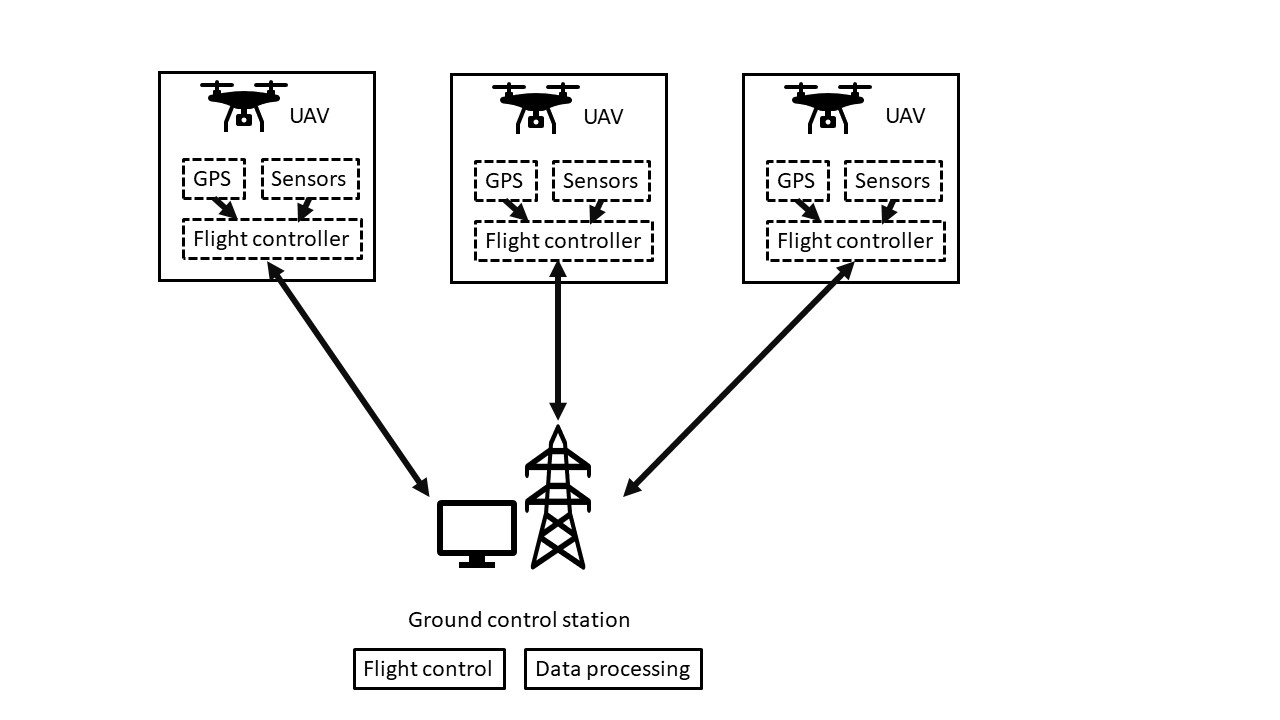
\includegraphics[width=1.2\linewidth]{images/infra.jpg}
\caption{Infrastructure-based swarm architecture}
\end{center}
\end{figure}
% === figure === %

\subsection{Flying Ad-hoc Network (FANET) Architecture}
\paragraph{}
Flying ad-hoc network (FANET) is the other commonly used communication architecture for UAV swarms. To exchange information, UAVs form a network that transfers messages in a hop-to-hop fashion, just like the traditional mobile ad-hoc network (MANET)\cite{6}. MANETs are composed of mobile nodes with random movements. A UAV swarm network can be considered as the aerial version of a MANET\cite{4}. MANET that are made of ground vehicles as mobile nodes are called Vehicular ad-hoc networks (VANETs). Flying ad-hoc network (FANET), is a subset of VANETs. They are composed of aerial vehicles. Figure 2.2 demonstrates the relationship between different ad-hoc networks. The connection of two devices in an ad-hoc network does not require the assistance of any other typical network infrastructure. However, one of the UAVs in the swarm must have access to a ground control station or a satellite\cite{doi:10.1139/juvs-2018-0009}. In recent years, researchers have shifted their focus from infrastructure-based swarm architecture to FANET due to its cheaper and simpler network deployment.  

%=== figure === %
\begin{figure}[h]
\begin{center}
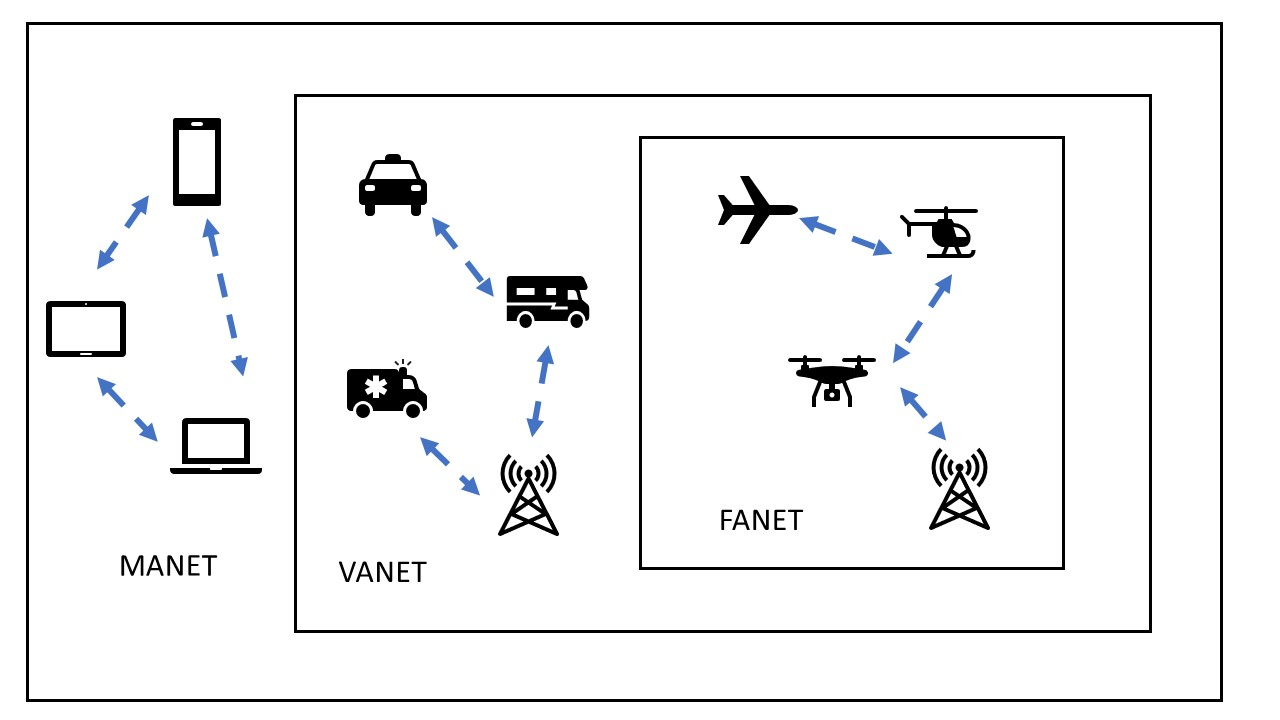
\includegraphics[width=1.05\linewidth]{images/adhoc.jpg}
\caption{Relationship of ad-hoc networks}
\end{center}
\end{figure}
% === figure === %

\paragraph{}
FANETs have also been studied under different names\cite{bekmezci2013flying}. Cameron {\it et al.}\cite{cameron2010suaave} named their autonomous UAV swarm as aerial robots. Their multi-UAV system communicates using 802.11 wireless ad-hoc and mesh networking. Another related research topic is aerial wireless sensor network\cite{ahmed2011link,ahmed2016importance, ahmed2013utilizing}. In aerial wireless sensor networks, multiple UAVs are equipped with various sensors to sense and collect information. The collected information can be forwarded to a faraway ground control station through an ad-hoc network in real-time.

\paragraph{}
FANETs are widely utilized in numerous applications, such as disaster monitoring and intelligent agriculture. Different applications have their own characteristics and demands. Developing high-performance and reliable protocols suitable for intended situations is important. The characteristics of UAV swarm network pose several unique challenges to the establishment and maintenance of an efficient UAV network. 

\section{The Challenges of UAV Swarm Networks}

\paragraph{}
Even though UAV networks share some common aspects with other kinds of ad-hoc network, it still has many unique design challenges. 

\subsubsection{Mobility}
\paragraph{}
The first challenge is the high mobility of UAVs. The nodes of UAV networks have relatively high moving speeds compared to MANET and FANET. The fast-changing topology makes the design of UAV networks an arduous work. The rapid movement of UAVs may disrupt ongoing transmissions as they move out of the transmission range. Link quality is unstable in UAV networks. Unlike VANETs where the node movement is generally restricted by 2D terrains, such as highways and roads, UAVs move freely in a 3D space. The altitude of flight must be considered to avoid collisions. In addition, the camera and sensors carried by UAVs have limited operating distances.\cite{Goodrich2008SupportingWS} states that although high altitudes give a larger view range, the sensors carried by UAV have limited accuracy, which does not allow the UAVs from flying too high in the sky. The moving direction and velocity of UAVs are frequently adjusted when the environment changes or mission updates. It is challenging to develop a generic mobility model that is suitable for every kind of UAV network simulation. 

\paragraph{}
In \cite{4124182}, two UAV mobility models for reconnaissance scenarios are proposed. UAVs move freely at random in the first model. The second model uses pheromones to guide the movement of UAVs, which provides outstanding scanning properties. However, it has problems concerning network connectivity. In \cite{7565125}, the authors present a distributed mobility model of autonomous UAV swarms for scouting application. It is the first UAV mobility model that includes the residual power level in decision making combined with area coverage and network connectivity. The authors of \cite{8855467} propose a 3D Smooth Random Walk (3DSRW) mobility model, which aims to profoundly simulate the three-dimensional movements of UAVs.

\subsubsection{Node Density}
\paragraph{}
UAV networks have a relatively low density than common ad-hoc networks. UAVs are usually dispersed in the sky. The operating range of sensors has grown larger as technology develops. For common aerial remote sensing applications, the UAVs are generally kilometers away from each other.

\subsubsection{Power Consumption}
\paragraph{}
In traditional MANETs, the node devices like cellphones and laptops usually have small lithium batteries. Because of the limited power capacity, power-efficient communication methods are important for the network to maximize the efficiency and lifespan\cite{lashari}. Similarly, small-size UAVs have the same characteristic. The emerging LASER technology also provides a solution to the problem as it allows battery recharging in space\cite{zhao2020efficiency}. 

\subsubsection{Localization}
\paragraph{}
The global positioning system (GPS) is widely used to spot outdoor devices in ad-hoc networks. The typical GPS receiver is accurate from 18 to 90 meters\cite{993780}, which is enough for common VANET applications. However, UAV network nodes move at high speed with more complex mobility patterns. They require very precise localization with extremely low latency\cite{lashari}. Advanced versions of GPS such as Differential GPS (DGPS) and assisted GPS (AGPS) are required to accurately locate UAVs promptly for UAV networks to work efficiently and reliably. Differential GPS enhances the accuracy to within one meter. AGPS enhances accuracy to less than 15 meters when users are outdoors. In addition, AGPS can retain information for privacy reasons, and the network administrator can limit access to intended users\cite{993780}.

\subsubsection{Computational power}
\paragraph{}
Small-size UAVs have energy and payload constraints. Their onboard computational performance is also limited. In infrastructure-based swarm architecture, the ground control station with high computational power provides necessary controlling functions and data processing abilities for the network. On the other hand, in FANETs, the nodes act as routers as ad-hoc communications do not require the assistance of additional infrastructures. Therefore, the UAVs must have required computational power to deal with collected information in real-time. Developing an efficient communication scheme for FANETs is very challenging with the limited computational power of small UAVs.

\section{Communication Protocols for UAV Swarms}
\paragraph{}
Many wireless are designated or suitable for UAV swarm applications. This section introduces the wireless communication technologies that have been used for UAV swarm communications.

\subsubsection{802.11}
\paragraph{}
The IEEE 802.11 series, known as Wi-Fi, utilize various unlicensed spectrum including, 2.4 GHz, 5 GHz, and etc. The 802.11a/b/g/n are the most commonly used protocols for ad-hoc networks. They guarantee an outdoor communication range of up to 150m with a maximum speed of 150 Mb/s. However, the standards only support movement speed up to 30m/s, which is not suitable for high-velocity UAV swarm applications\cite{chen2020toward}. In 2017, IEEE 802.11ah technology, Wi-Fi CERTIFIED HaLow, is designed for IoT applications. It operates in spectrum below 1 gigahertz (GHz) to offer extended communication range and lower power connectivity. IEEE 802.11ah also supports MIMO\cite{Shi_2021}

\subsubsection{3GPP Cellular Networks}
\paragraph{}
The Third Generation Partnership Project (3GPP) standards are the globally applicable technical specifications for cellular networks. Long Term Evolution - Advanced (LTE-A) provides low latency and high data rates. However, cellular networks typically utilize licensed spectrums, which limits their applications\cite{chen2020toward}. The currently developing 5G networks have the potential for even faster UAV communications utilizing mmWave bands.

\subsubsection{ZigBee}
\paragraph{}
The IEEE 802.15.4 standard, namely ZigBee, is widely used for UAV accessories. The IEEE 802.15.4 standard is designed for power-efficient low-cost D2D communications\cite{Shi_2021}. Nonetheless, the data rates of ZigBee products are often lower than the Wi-Fi family. Its data rate of 250 kb/s cannot satisfy applications that make high Quality of Service (QoS) demands.

\section{Design of UAV Swarm Network Routing Protocols}

\paragraph{}
In the early days, MANET and VANET routing protocols were widely adapted in UAV network testbeds\cite{8772093}. The researchers soon realized MANET and VANET routing protocols are not suitable for UAV networks due to the special characteristics of drones, especially their rapidly changing flying patterns. UAV swarm routing protocols attract more research interest recently. Routing protocols of UAV networks can be categorized into Topology-based Routing Protocols and Geographical Routing Protocols\cite{8772093}. Figure 2.3 shows the categories of UAV network routing protocols.

%=== figure === %
\begin{figure}[h]
\begin{center}
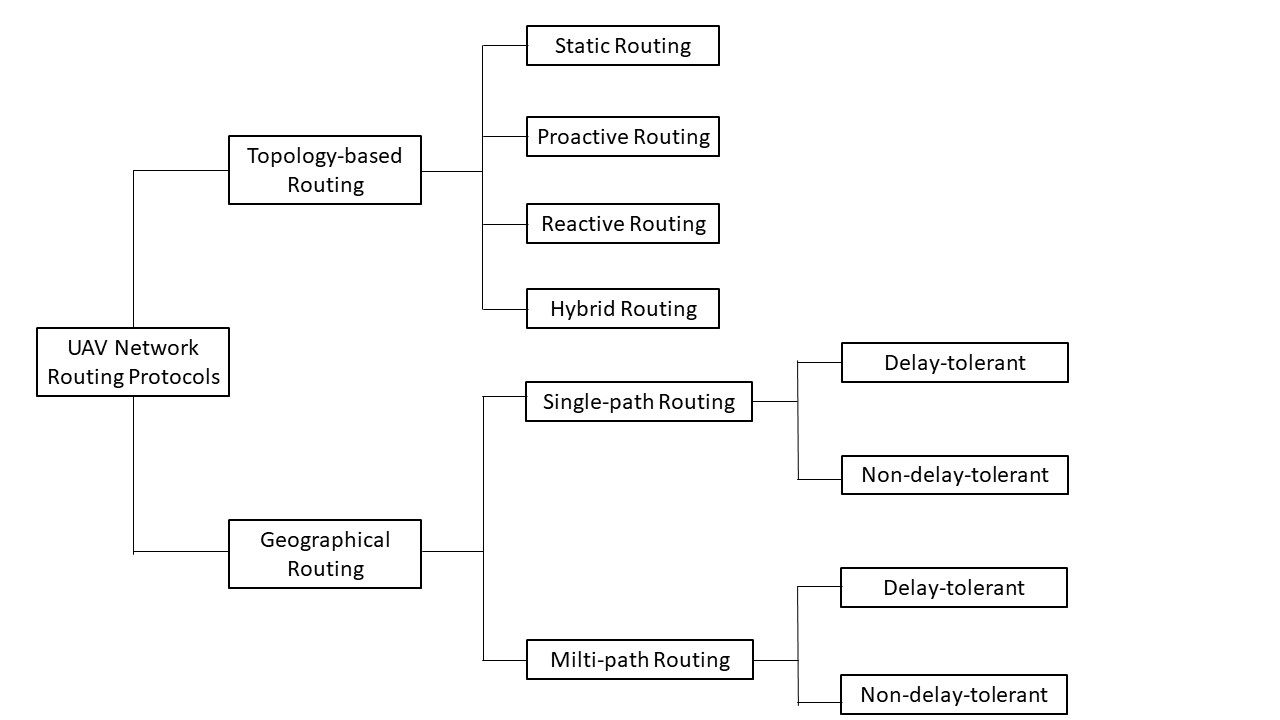
\includegraphics[width=1.05\linewidth]{images/routing.jpg}
\caption{Categories of UAV network routing protocols}
\end{center}
\end{figure}
% === figure === %

\subsection{Topology-based Routing Protocols}
\paragraph{}
Topology-based Routing Protocols exploit the information of links between UAVs to decide the path of transmission. The protocols use IP addresses to distinguish different nodes. Owing to the highly mobility of UAV swarms, designing Topology-based Routing Protocols is very challenging as the topology changes rapidly and frequently.

\paragraph{}
Topology-based Routing Protocols are further classified into four categories: static routing, proactive routing, reactive routing, and hybrid routing\cite{8772093}.

\subsubsection{Static Routing}
\paragraph{}
Static routing protocols maintain a fixed routing table that is generated and stored in the system prior to the mission. The routing table cannot be modified or updated during the mission. Therefore, the protocols are fault-intolerant\cite{Yanmaz2018DroneNC}. They do not function normally when link failure happens.

\paragraph{}
Data-Centric Routing (DCR) is a static routing protocol for multicast communications. It transfers data when the data is requested by a group of nodes at the same time. DCR works better in clustered UAV networks to provide applications that disseminate particular data for an explicit mission area\cite{topobased}.

\paragraph{}
Load Carry and Deliver Routing (LCAD) is a also static routing mechanism for FANETs. Before the mission begins, UAVs are loaded with data from a ground control station. LCAD manages the flight route for the UAVs to carry and deliver the messages to the destination ground control station. The protocol is often used for delay-tolerant tasks. This method is safe and has efficient\cite{kung2008research, Yanmaz2018DroneNC, topobased}, but the delay is high as the communicating ground stations are far from each other.\cite{kung2008research, Yanmaz2018DroneNC, topobased}.

\paragraph{}
Another common static routing protocol is Multi-Level Hierarchical Routing (MLHR). The hierarchical structure is designed to expand the operation area and size, which mitigates the scalability problem of large-scale UAV swarm network\cite{guillen2021comparative}. In a hierarchical network, clusters are formed for specific functions. Every cluster has a single Cluster Head. Only the Cluster Heads have direct links to other Cluster Heads and the ground control station.

\subsubsection{Proactive Routing Protocol (PRP)}
\paragraph{}
Proactive Routing Protocols (PRP) maintain a dynamic routing table, which is distributed and updated among all the UAVs periodically. Proactive Routing Protocols usually have the updated data. However, the frequent update of network status may consume too much bandwidth. It shows significant delay when topology changes\cite{7995044}.

\paragraph{}
Optimized link-state routing (OLSR) is a popular proactive routing method used in ad-hoc networks\cite{8772093}. It is a proactive routing protocol where Multi-point relay (MPR) nodes update the link status of their neighbors via HELLO messages periodically. The protocol chooses optimal forwarding links to transfer the message. Overhead is created while exchanging the HELLO messages. In \cite{5}, Chen {\it et al.} proposed a proactive broadcast algorithm using the neighbor quality-based MPR mechanism for FANET. In their scheme, each node collects its local neighbors' physical link condition and congestion level via HELLO message. The rebroadcast decision is made based on the link quality of its neighbors, which are calculated using Received Signal Strength Indication (RSSI) and MAC layer length of a node. They select less busy nodes as a relay to avoid congestion and reduce the number of rebroadcasts.

Based on the mechanism of OLSR, Optimized Link Routing With Expected Transmission Count (OLSR-ETX) is developed\cite{Xie2018AnEO}. The author in \cite{Xie2018AnEO} utilizes the nodes' GPS positions to calculate link life-time. The system makes decisions based on the remaining energy of potential forwarding nodes. \cite{8772093} states that "OLSR-ETX performs better than the traditional OLSR in terms of packet transmission, end-to-end delay, and overhead."

\subsubsection{Reactive Routing Protocol (RRP)}
\paragraph{}
Reactive Routing Protocols (RRPs) are the protocols that provide on-demand routing services. The path of the two nodes is calculated and stored only when data transmission is requested. The goal of Reactive Routing Protocols is to mitigate the drawbacks of frequent updates in Proactive Routing Protocols.

\paragraph{}
Ad-Hoc On-Demand Distance Vector (AODV) is an on-demand reactive routing protocol. It determines the path when the source requests a message transfer and keeps the information if the source desires. To discover a path to the destination, the source node advertises a route request (RREQ) packet. Relay nodes along the path forward RREQ and store the frame information\cite{maurya2012overview}. If routing fails, a route error packet (RERR) message is created to tell the source node about the error so that the source can re-initiate the process. AODV dynamically adjusts link status, memory usage, and other resource utilization\cite{maurya2012overview}.

\paragraph{}
A variation of the AODV called Radiometric Ad-Hoc On-Demand Distance Vector (RM-AODV) is proposed by the IEEE 802.11s standard\cite{topobased}. RM-AODV eliminates the complexity of the route discovery from the upper layers so that they see all nodes one single hop away\cite{topobased}. The protocol evaluates both the link quality and the amount of resources required when a frame is transmitted via a particular route. NS3-Evalvid simulation results indicated that RM-AODV improves the network performance by delivering better latency, packet success rate, overhead cost, and the peak-signal-to-noise ratio of the received video\cite{katila2017routing}.

\paragraph{}
Other Reactive Routing Protocols includes adaptive density-based routing protocol (ADRP)\cite{zheng2017adaptive}, Dynamic Source Routing (DSR)\cite{alshabtat2011low}, Self Adaptive Routing Protocol (SARP)\cite{elwhishi2009sarp}, etc.

\subsubsection{Hybrid Routing Protocol (HRP)}
\paragraph{}
Hybrid Routing Protocols overcome the disadvantages of both Reactive Routing Protocols and Proactive Routing Protocols by combining their advantages\cite{topobased}. Traditional hybrid routing protocols exploit the concept of zones\cite{haas2001zone, wang2004two}. Nodes are divided into zones and proactive method is deployed within the zones to reduce overhead. For communication across zones, reactive strategy is applied. 

\paragraph{}
Temporarily Ordered Routing Algorithm (TORA) is a hybrid routing protocol for multi-hop networks where routes only keep data of neighbor UAVs to minimize the influence of topology changes\cite{8772093}. It is based on the concept of link reversal\cite{gupta2010performance}. TORA protocol keeps more than one path to the destination. The protocol only re-configures when all paths fail.

\paragraph{}
In \cite{li2017lepr}, Li and Yan propose a hybrid protocol for FANET, namely Link Stability Estimation-based Preemptive Routing (LEPR). LEPR uses the link quality, safety degree, and mobility prediction factor to take into account the past, current, and future statuses of link stability respectively. A semi-proactive route maintenance process is initiated when a link failure occurs.

\subsection{Geographical/Position-based Routing Protocols}
\paragraph{}
Geographical/Position-based Routing Protocols are based on GPS information of the nodes. This routing is perfect for highly dynamic UAV communication networks. Position-based routing can be classified into two categories: single-path-based, and multi-path-based. Both single- and multi-path-based routing protocols are categorized further into heterogeneous networks, delay-tolerant networks (DTNs), and non-delay-tolerant networks (Non-DTNs)\cite{8772093}. As this paper is focused on UAV swarm networks, heterogeneous networks will not be discussed. 

\subsubsection{Single-Path Delay-Tolerant Network Routing (DTN)}
\paragraph{}
DTN protocols utilize store-carry-and-forward. DTN protocols store the data packets until they are transferred to another UAV, which makes them fault-tolerant.

\paragraph{}
Kuiper and Nadjm-Tehrani\cite{5634136} propose Location-Aware Routing for Opportunistic Delay-Tolerant Networks (LAROD), a delay-tolerant geographical routing protocol that is based on the combination of greedy forwarding and store-carry-and-forward methods. Messages are transmitted through broadcasting. If the message is not received by any other node, the source node intermittently re-broadcasts the message until a node becomes available in the network. Store-carry-and-forward methods hold the data packets until they reach the destination. LAROD is an energy-consuming protocol, which is not suitable for small-size UAVs.

\subsubsection{Single-Path Non-Delay-Tolerant Network Routing}
\paragraph{}
Non-DTN routing protocols are suitable for high-density UAV swarm network. They are divided into greedy-based and reactive-based protocols\cite{8772093}. Greedy-based protocols transmit messages to the closest neighbors to forward the target destinations. However, message transfer may fail if there are not adjacent nodes, and a backup plan may be needed\cite{8772093}. Reactive-based protocols require to have a complete route to the destination based on routing paths. .

\paragraph{}
In \cite{8553810}, the authors introduce a reliable UAV single-path non-delay-tolerant communication routing using the Global Positioning System (GPS) with improved Optimized Link State Routing Protocol (i- OLSR). Link quality estimation and speed weighted Expected Transmission count (ETX) are calculated for the pursue mobility model to provide efficient routing.

\subsubsection{Multi-Path Non-Delay-Tolerant Network Routing}
\paragraph{}
Numerous Non-DTN routing protocols based on geographical information have been proposed. Shirani {\it et al.} \cite{shirani2012delay} present Reactive-Greedy-Reactive (RGR), a routing protocol in highly mobile density-variable UAV networks. In the Greedy Geographic Forwarding (GGF) part of RGR, a node is chosen for packet forwarding based on its distance to the destination node. If no available path to the destination is discovered, then the source node must initiate an on-demand route to maintain the communication with the target node.

\paragraph{}
Choi {\it et al.} \cite{8436724} propose Geographical Routing Protocol for UAV networks with multi-hop communication. Their protocol uses geolocation information of neighbor nodes and determines the routing path to the destination by only considering the neighbor information, which in turn, results in low overhead and robustness to the dynamic network topology in FANETs. 

\subsubsection{Multi-Path DTN Routing}
\paragraph{}
In \cite{8490824}, Arafat and Moh propose a location-aided delay tolerant routing (LADTR) protocol for UAV networks for post-disaster applications, which utilizes Global Positioning System guided routing combined with a store-carry-forward (SCF) mechanism. They proposed Ferrying UAVs to improve SCF.  Ferrying UAVs enhance the availability of links between the probing UAVs and the ground control station, which lowers end-to-end delays and improves the packet delivery ratio\cite{8490824}. 

\paragraph{}
Pu \cite{8523684} propose a jamming-resilient multi-path non-delay-tolerant protocol called JarmRout. JarmRout utilizes a combination of three major schemes which are link quality scheme, traffic load scheme, and spatial distance scheme to avoid network failures caused by intentional jamming and disruption.

\paragraph{}
The communication mechanism for UAV swarms can be extremely complex and routing protocols are hard to design. Similar to traditional networks, UAV communications can be categorized into unicast, multicast, and broadcast. Unicast is the hop-to-hop information exchange between two nodes. Multicast communications maintain a network structure such as a tree or a mesh structure. It utilizes the network structure to deliver messages from one single node to a group of destination nodes. In Broadcast communications, messages are disseminated over the entire network. The deployment for broadcast is relatively cheap and simple. As UAVs have limited resources, broadcasting is efficient and suitable for UAV swarm communication. 

\paragraph{}
Flooding is the traditional and the simplest way of broadcasting messages to all the nodes in a network\cite{flooding}. In the conventional flooding scheme, when a node receives a new packet, it disseminates the packets to its neighbors. The rebroadcast behavior continues until all of the nodes in the network receive the packet. However, in a large-scale UAV swarm network, simple flooding triggers a massive number of packet transmissions causing serious contentions and collisions, which may eventually overwhelm the network and depletes the already limited resources of UAVs~\cite{tseng2002broadcast}. Therefore, it is crucial to employ efficient broadcast protocols to maintain the coordination of the UAV swarm. 

\paragraph{}
Qin {\it et al.}\cite{6} improve the traditional probabilistic rebroadcast technique using reinforcement learning. Each node forecasts the probability of collision and contention based on the network topology dynamically and evaluates the reward of rebroadcasting actions to determine forwarding probability dynamically. Their scheme aims to adapt to the high mobile UAV networks.

\paragraph{}
In \cite{9531630}, they mitigate the BSP by calculating the score of each node before rebroadcast. The score is derived from movement direction, residual energy, link quality, and node stability. The packets are only re-transmitted when the score of the received node exceeds a designated threshold. 

\paragraph{}
From the physical layer perspective, \cite{beamforming} designed a lightweight beamforming algorithm, which uses beams to predict the movements of UAVs. They utilize beamforming to overcome the inherent position error. The algorithm significantly improves uplink transmission performance and thus decreases the costs of resources.

\paragraph{}
To reduce the broadcast costs and performance, most researchers focus on mitigating the Broadcast Storm Problem by limiting the number of re-transmissions. Some others provide physical layer solutions. Our paper, on the other hand, investigate the performance of skeleton framework and greedy-based source selection algorithms in UAV swarm broadcast communications. We also adapt two greedy-based source algorithms to simplify the skeleton framework, which will be described in detail in the next chapter.


\chapter {Methodology}

%*------------------------------------------------------
\paragraph{}
In this chapter, we introduce the the star-like skeleton-based framework of \cite{ssr} and greedy-based algorithms proposed in \cite{prose}, and describe how we adapt the algorithms to modify the skeleton. In addition, the network and system assumptions in which we conduct performance investigations are provided.

\section{The Skeleton Framework}
%=== figure === %
\begin{figure}[tbph]
\begin{subfigure}{.5\textwidth}
  \centering
  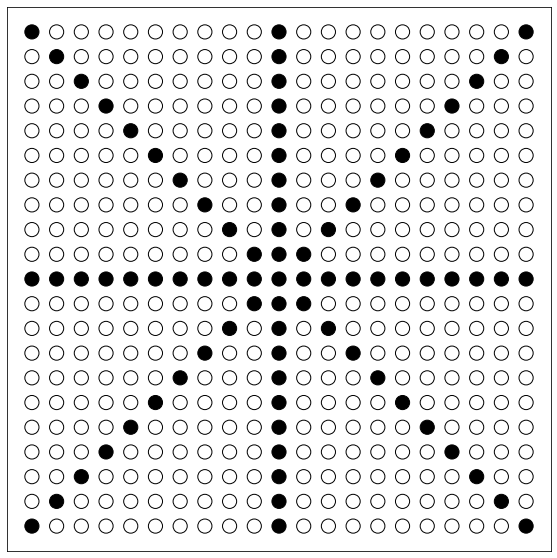
\includegraphics[width=.8\linewidth]{images/square.png}
  \caption{Square fly formation}
  \label{fig:sfig1}
\end{subfigure}%
\begin{subfigure}{.5\textwidth}
  \centering
  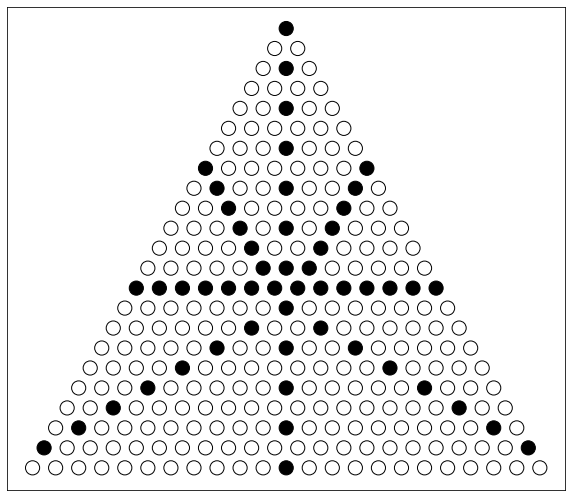
\includegraphics[width=.8\linewidth]{images/triangle.png}
  \caption{Triangular fly formation}
  \label{fig:sfig2}
\end{subfigure}
\caption{Star-like skeleton framework}
\label{fig:fig}
\end{figure}
% === figure === %
\paragraph{}
In \cite{ssr}, the skeleton framework is used to utilize the limited UAV network resource during unicast communications. The skeleton of in \cite{ssr} refers to the stable nodes located in the critical positions of the fix-shape UAV swarm formation. Since the resources of the UAV network are limited, control messages and topology information are only stored in or transmitted to the skeleton nodes by the ground control station, which reduces communication overhead and resource consumption. Other regular nodes have no direct access to the ground control station.

\paragraph{}
The authors of \cite{ssr} employ star-like skeleton structures in their routing scheme to distribute messages fast and uniformly. The skeleton nodes also help the UAV swarm change formation shape and provide a convenient way of addressing the nodes in a 2D coordinate system. However, the skeleton node selection in \cite{ssr} takes unicast routing and formation morphing into consideration, which leads to too many redundant broadcast source nodes if used for efficient broadcast schemes. Therefore, in this paper, we adapt the source selection algorithms from \cite{prose} to simplify the star-like skeletons, making them suitable for resource-efficient fixed-shape UAV swarm broadcast schemes.

\section{Network and System Assumptions}

\subsection{Node Mobility and Topology}
\paragraph{}
UAV networks are generally described as highly dynamic with rapid changing topology~\cite{ssr}. Nevertheless, in many applications, such as drone light shows and aerial mapping, UAVs spend a large portion of time in fixed-shape swarm formations during the mission. In this study, we investigate the performance of the UAV swarm that remains static in a 2-D fixed-shape topology.

\subsection{Node Resources}
\paragraph{}
The UAV swarm system does not require precise GPS information. It only relies on relative positions. The nodes estimate the angle and distance of their neighbors by using RSS-related methods or other simple sensors/cameras. The UAVs have limited battery power and computational ability. The essential command messages or topology information can be either pre-loaded or sent by the ground control stations to the skeleton nodes. Only the skeleton nodes have access to commands. They serve as initial broadcast sources to disseminate essential information to all the other nodes in the UAV swarm network.




\section{The Greedy-based Source Selection Algorithms}

\paragraph{}
In~\cite{prose}, Sou {\it et al.} proposed two greedy-based broadcast source selection algorithms, Greedy and Defer, to reduce broadcast costs of file distribution in post-disaster scenarios. They designed the algorithms using the Minimum Connected Dominating Set concept, trying to minimize the number of broadcast sources needed. 

\paragraph{}
Let an unweighted graph $G(V, E)$ represent the topology of the UAV swarm formation with star-like skeleton nodes, as shown in Figure 3.1. V denotes the set of nodes, and E represents the set of edges between one-hop neighbors. Each node is either black or white. Black vertices represent the nodes that already possess the message. The skeleton nodes are initially black, as they are the only nodes with access to commands and mission information, either pre-loaded or received from the ground control station. The skeleton nodes serve as the initial sources to broadcast the message to the entire network. Other nodes waiting to receive the message are colored white. We use the graph as input to the source selection algorithms. 

\paragraph{}
Let $S$ represent the set of sources selected and $w(x)$ be the set of white neighbors of node $x$. We assume all $x \in S$ transfer the message to their neighbors $w(x)$ using broadcast. Considering only one-hop neighbors each iteration, the source selection algorithms iteratively select suitable black nodes as sources and add them to $S$. Then the neighbors of the selected sources are colored black indicating the reception of the message. The process repeats until all the nodes are black.


\subsection{Greedy}

\paragraph{}
The Greedy algorithm by \cite{prose}, as its name implies, always makes the locally optimal decision each round. Considering only the one-hop neighbors during each iteration, the algorithm adds the black nodes that can cover the maximum white neighbors to $S$. The source selection process repeats until all the nodes are black. However, local optimalities do not always yield the best global result~\cite{prose}. Sou {\it et al.}\cite{prose} proposed the Defer algorithm to further reduce the number of broadcasts.

\subsection{Defer}

\paragraph{}
The Defer algorithm\cite{prose} improves the Greedy algorithm by taking all potential sources and subsequent transmissions into consideration. During each iteration, it first uses Greedy to obtain a set of candidate nodes $C$. A candidate $x \in C$ is selected as a source if and only if all of its one-hop white neighbors can only receive the message from $x$. If all white neighbors of $x$ can potentially receive the message from other black nodes or later from subsequent retransmissions, $x$ is not added to $S$. In order to track potential subsequent transmissions, when a node is added to $S$, its white neighbors are colored gray, as described ion line 22 to 23 of Algorithm 3. In other words, they are the candidates of the next iteration.

%========== Algorithm ==========%

    \begin{algorithm}
    \caption{Adapted Greedy}\label{euclid}
    \hspace*{\algorithmicindent} \textbf{Input:} $\textit G(V, E)$
    \hspace*{\algorithmicindent} \textbf{Output:} $\textit i, S$
    \begin{algorithmic}[1]
    \BState $V' \gets \emptyset$
    \BState $B' \gets V$
    \BState \textbf{Remove all $x \in B'$ that is white}
    \BState \textbf{Remove all $x \in B'$ that has no white neighbor}
    \BState $S \gets \emptyset$, $S' \gets \emptyset$,  $i \gets 1$
    \While {$x \in B'$ has white neighbor}
        \State $B \gets B'$, $B' \gets \emptyset$, $S' \gets \emptyset$
        \For {\texttt each node $x \in B$}
            \State $R \gets R \cup w(x)$
        \EndFor
        \While {$R \neq \emptyset$}
            \State {$x \gets arg max_{x \in B} |w(x)|$}
            \State {$S \gets S \cup \{x\}$, $S' \gets S' \cup \{x\}$, $B \gets B-\{x\}$}
            \State {Color the nodes in set w(x) black}
            \State {$R \gets R - w(x)$, $B' \gets B' \cup w(x)$}
        \EndWhile
        \If {$i = 1$}
            \State {$V' \gets V' \cup S'$}
            \EndIf
        \State {$i \gets i+1$}
    \EndWhile
    \If {$V' \neq \emptyset$}
        \State {$V' \gets V' \cup S'$}
        \For {\texttt each node $v \in V$}
            \If {$v \notin V'$}
                \State {Color v white}        
            \EndIf
        \EndFor
        \State {Go to line 2}
    \EndIf
    \end{algorithmic}
    \end{algorithm}
%========== Algorithm ==========%    
    
    \begin{algorithm}
    \caption{Adapted Defer}\label{euclid}
    \hspace*{\algorithmicindent} \textbf{Input:} $\textit G(V, E)$
    \hspace*{\algorithmicindent} \textbf{Output:} $\textit i, S$
    \begin{algorithmic}[1]
    \BState $V' \gets \emptyset$
    \BState $S \gets \emptyset$, $S' \gets \emptyset$,  $i \gets 1$
    \BState \textbf{Use Greedy to find out $C$; go to line 25 if $C = \emptyset$}
    \If{$C = \emptyset$}
        \If {$i=1$} { $V' \gets V' \cup 'S$}
        \EndIf
        \State {$i \gets i+1$, $S' \gets \emptyset$}
        \State {Go to line 3}
    \Else
        \State {$x' \gets arg min_{x \in C} |w(x')|$}
        \State {$T \gets w(x')$}
    \EndIf
    \If {$T = \emptyset$}
        \State {Go to line 4}
    \Else 
        \State {Select a node n from T}
    \EndIf
    \If {n has other black neighbor} {go to line 11}
    \EndIf
    \If {n does not have gray neighbor} {go to line 21}
    \EndIf
    \If {exists a node $r \in w(n)$ has no other black and gray neighbor}
        \State {Go to line 21}
    \Else
        \State {Go to line 11}
    \EndIf
    \For {each $n \in w(x')$}
        \State {color n gray}
        \State {$S \gets S \cup x'$, $S' \gets S' \cup x'$}
        \State {Go to line 4}    
    \EndFor
    \If {$V' \neq \emptyset$}
        \State {$V' \gets V' \cup S'$}
        \For {\texttt each node $v \in V$}
            \If {$v \notin V'$}{ color v white}  
            \EndIf
        \EndFor
        \State {Go to line 2}
    \EndIf    
    \end{algorithmic}
    \end{algorithm}
    
%========== Algorithm ==========%   


\newpage
\section{Modifying the skeleton}

\paragraph{}

%=== figure === %
\begin{figure}[h]
\begin{center}
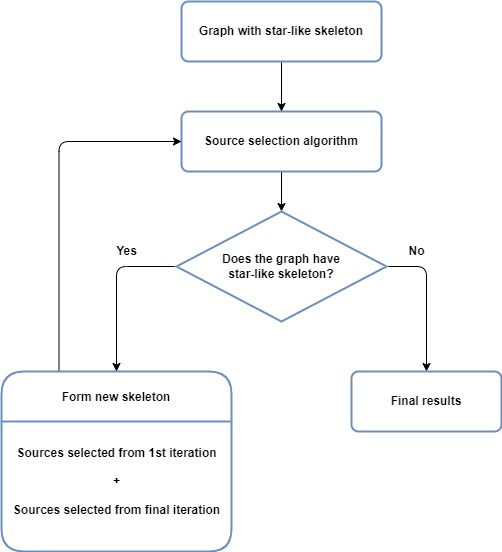
\includegraphics[width=5in]{images/flow_chart.jpg}
\caption{Skeleton simplification}
\end{center}
\end{figure}
% === figure === %

\paragraph{}
As mentioned in the previous section, the star-like skeletons are not cost-efficient in broadcast scenarios. To effectively reduce the broadcast costs, we adapt the algorithms from \cite{prose} to simplify the star-like skeleton structures from \cite{ssr}. This section explains in detail how we modify the skeletons.  Fig 3.2 presents a flowchart of the process. The pseudo-codes of the modified algorithms are shown as Algorithm 1 and Algorithm 2.

\paragraph{}
First, the original graph of topology with star-like skeleton is used as input to the source selection algorithm. After running the algorithm once, according to its result, we replace the star-like skeleton with the nodes selected during the first and the final iteration to form a new simplified skeleton structure. Finally, we repeat the source selection process using the simplified skeleton and obtain the ultimate result.

\paragraph{}
Since the skeleton nodes have extensive access to a larger portion of resources and are used as the candidates for the initial broadcasts, it is not necessary to have them as skeleton if they are not selected during the first iteration. Removing them releases resources back to the network and reduces overall communication overhead. Moreover, as observed in the last few iterations, there are usually only a few sparse white nodes left which require extra transmissions. If we take care of the nodes first, adding the sources selected during the last iteration to the skeleton will reduce the number of broadcast iterations. Above are the reasons we run the source selection algorithm once to replace the star-like skeleton the sources selected from the first and the last iteration.

%=== figure === %
\begin{figure}[tbph]
\begin{center}
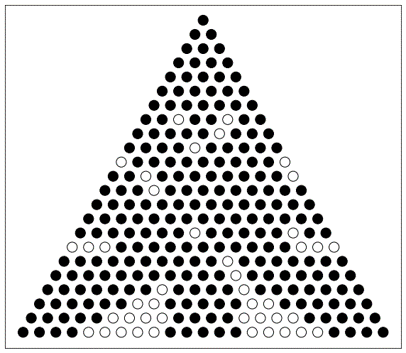
\includegraphics[width=.55\linewidth]{images/sparse.png}
\caption{The sparse white nodes during the last few iterations.}
\end{center}
\end{figure}
% === figure === %







%*------------------------------------------------------
\chapter{Experimental Evaluation}

\paragraph{}
This chapter shows the experimental evaluations of the Greedy and Defer algorithms on the star-like skeleton framework, and the simplified skeletons. 


\section{Experimental setups}
\paragraph{}We apply the adapted Greedy and Defer algorithm to the square and triangular swarm formations with star-skeleton structures as illustrated in Figure 3.1. Then we compare the performance differences between the star-like skeleton and the skeleton simplified in broadcast communications. 

\paragraph{}
The experiments with square swarm formation are performed with three different group sizes, i.e. 121, 225, and 289 nodes. The experiments with triangular formation use group sizes of 190, 231, and 276 nodes.

\paragraph{}
In our experiments, we assume the nodes are arranged with a fixed distance between them. The transmission rage of a node $V1$ is set to cover the eight adjacent nodes around it, including the diagonal ones. That means if the fixed space between nodes has a unit distance of $1$, the transmission radius of nodes is $\sqrt{2}$. Figure 4.1 illustrates the eight one-hop neighbors of $V_1$, which includes $V_2$-$V_8$. 

\paragraph{}
%=== figure === %
\begin{figure}
\begin{center}
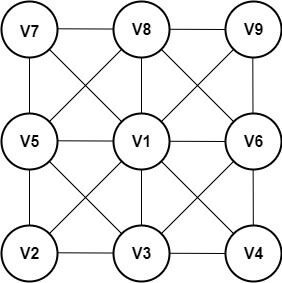
\includegraphics[width=.35\linewidth]{images/range.jpg}
\caption{The transmission range of node $V_1$ contains the 8 surrounding nodes $V_2$-$V_8$.}
\end{center}
\end{figure}
% === figure === %

\section{Results and analysis}
\paragraph{}
The results are analyzed using two metrics: the number broadcast nodes selected, and the number of broadcast iterations required for the entire UAV swarm network to receive the message.

\subsection{Comparison of skeleton size}

\paragraph{}
As mentioned in Section 3.1, skeleton nodes have access to an extensive amount of resources. Thus, selecting only the most essential nodes to minimize the size of the skeleton can significantly reduce communication overhead and resource consumption. Figure 4.2 shows the sizes of the star-like skeletons and the ones simplified based on the first round and final round results of the Greedy and Defer algorithms. Defer algorithm requires fewer skeleton nodes than Greedy. Moreover, the results indicate that our proposed method of simplifying the star-like skeleton can reduce the skeleton nodes up to approximately 56.9\%.
\paragraph{}
%=== figure === %
\begin{figure}[tbph]
    %\centering
    \begin{subfigure}{1\linewidth}
    \centering
        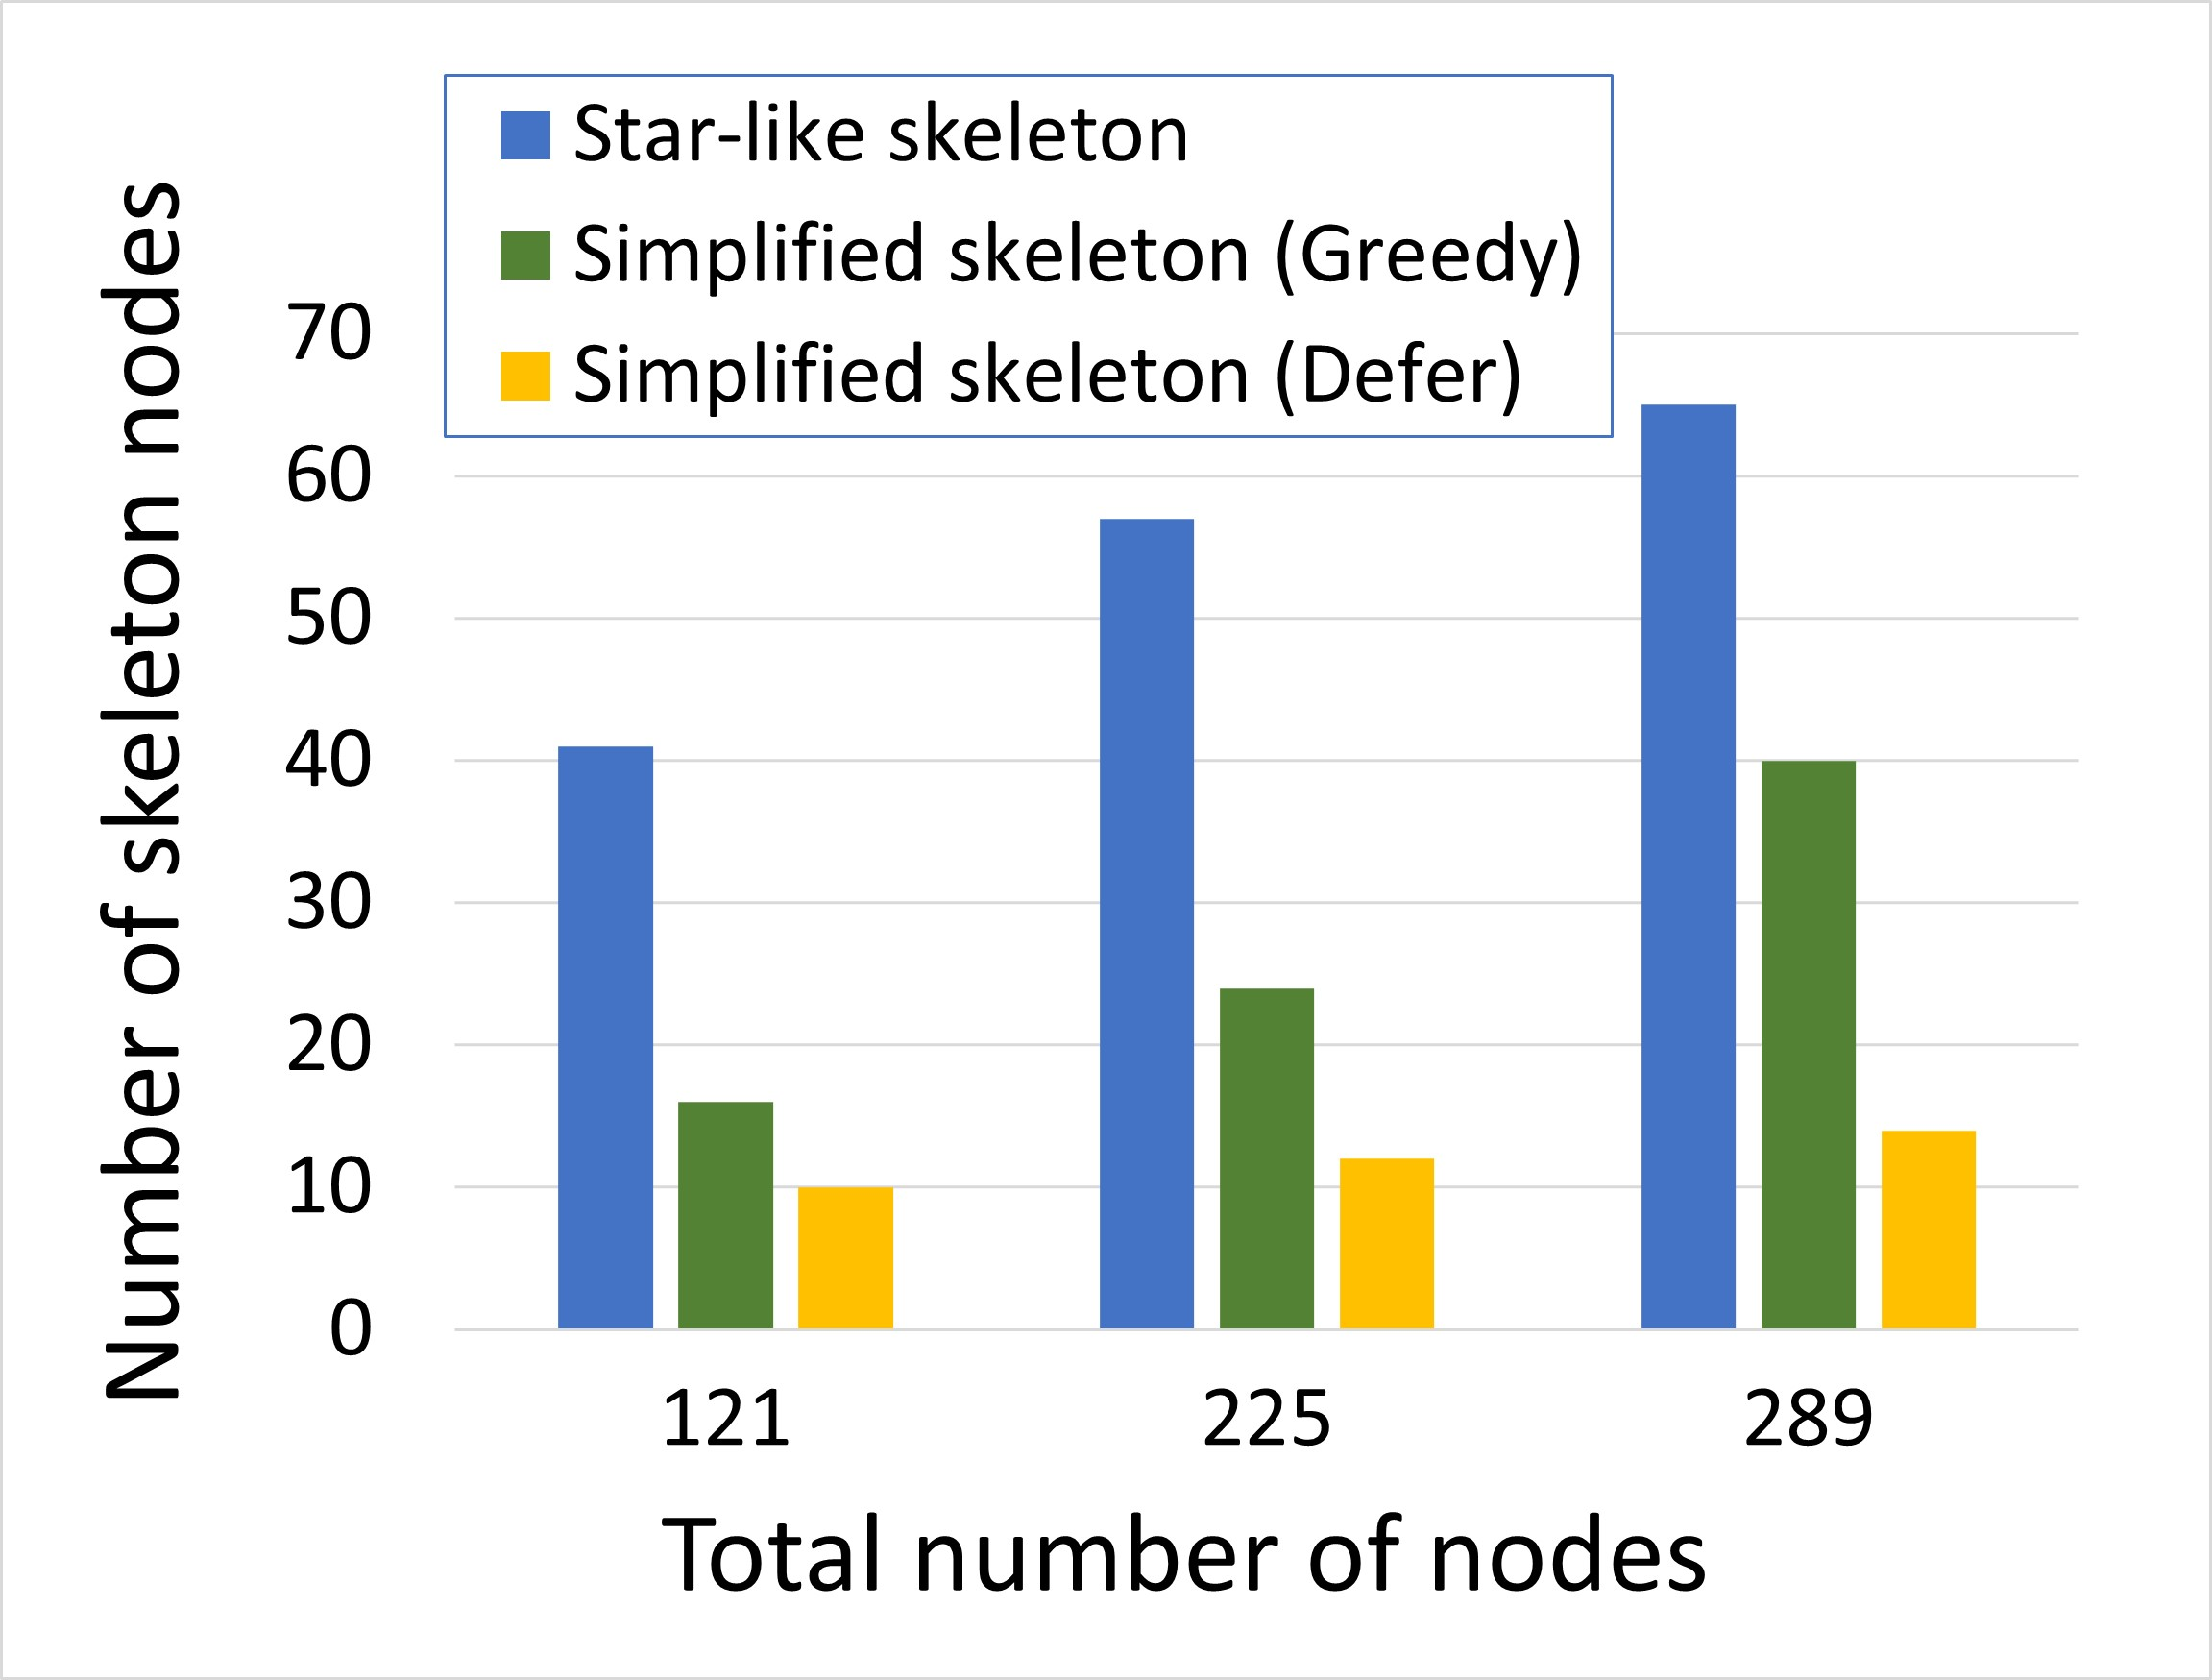
\includegraphics[width=0.8\textwidth]{images/results_skeleton_square.jpg}
        \caption{Square swarm formation}
    \end{subfigure}
    
    \vspace{1cm}
    \begin{subfigure}{1\linewidth}
    \centering
        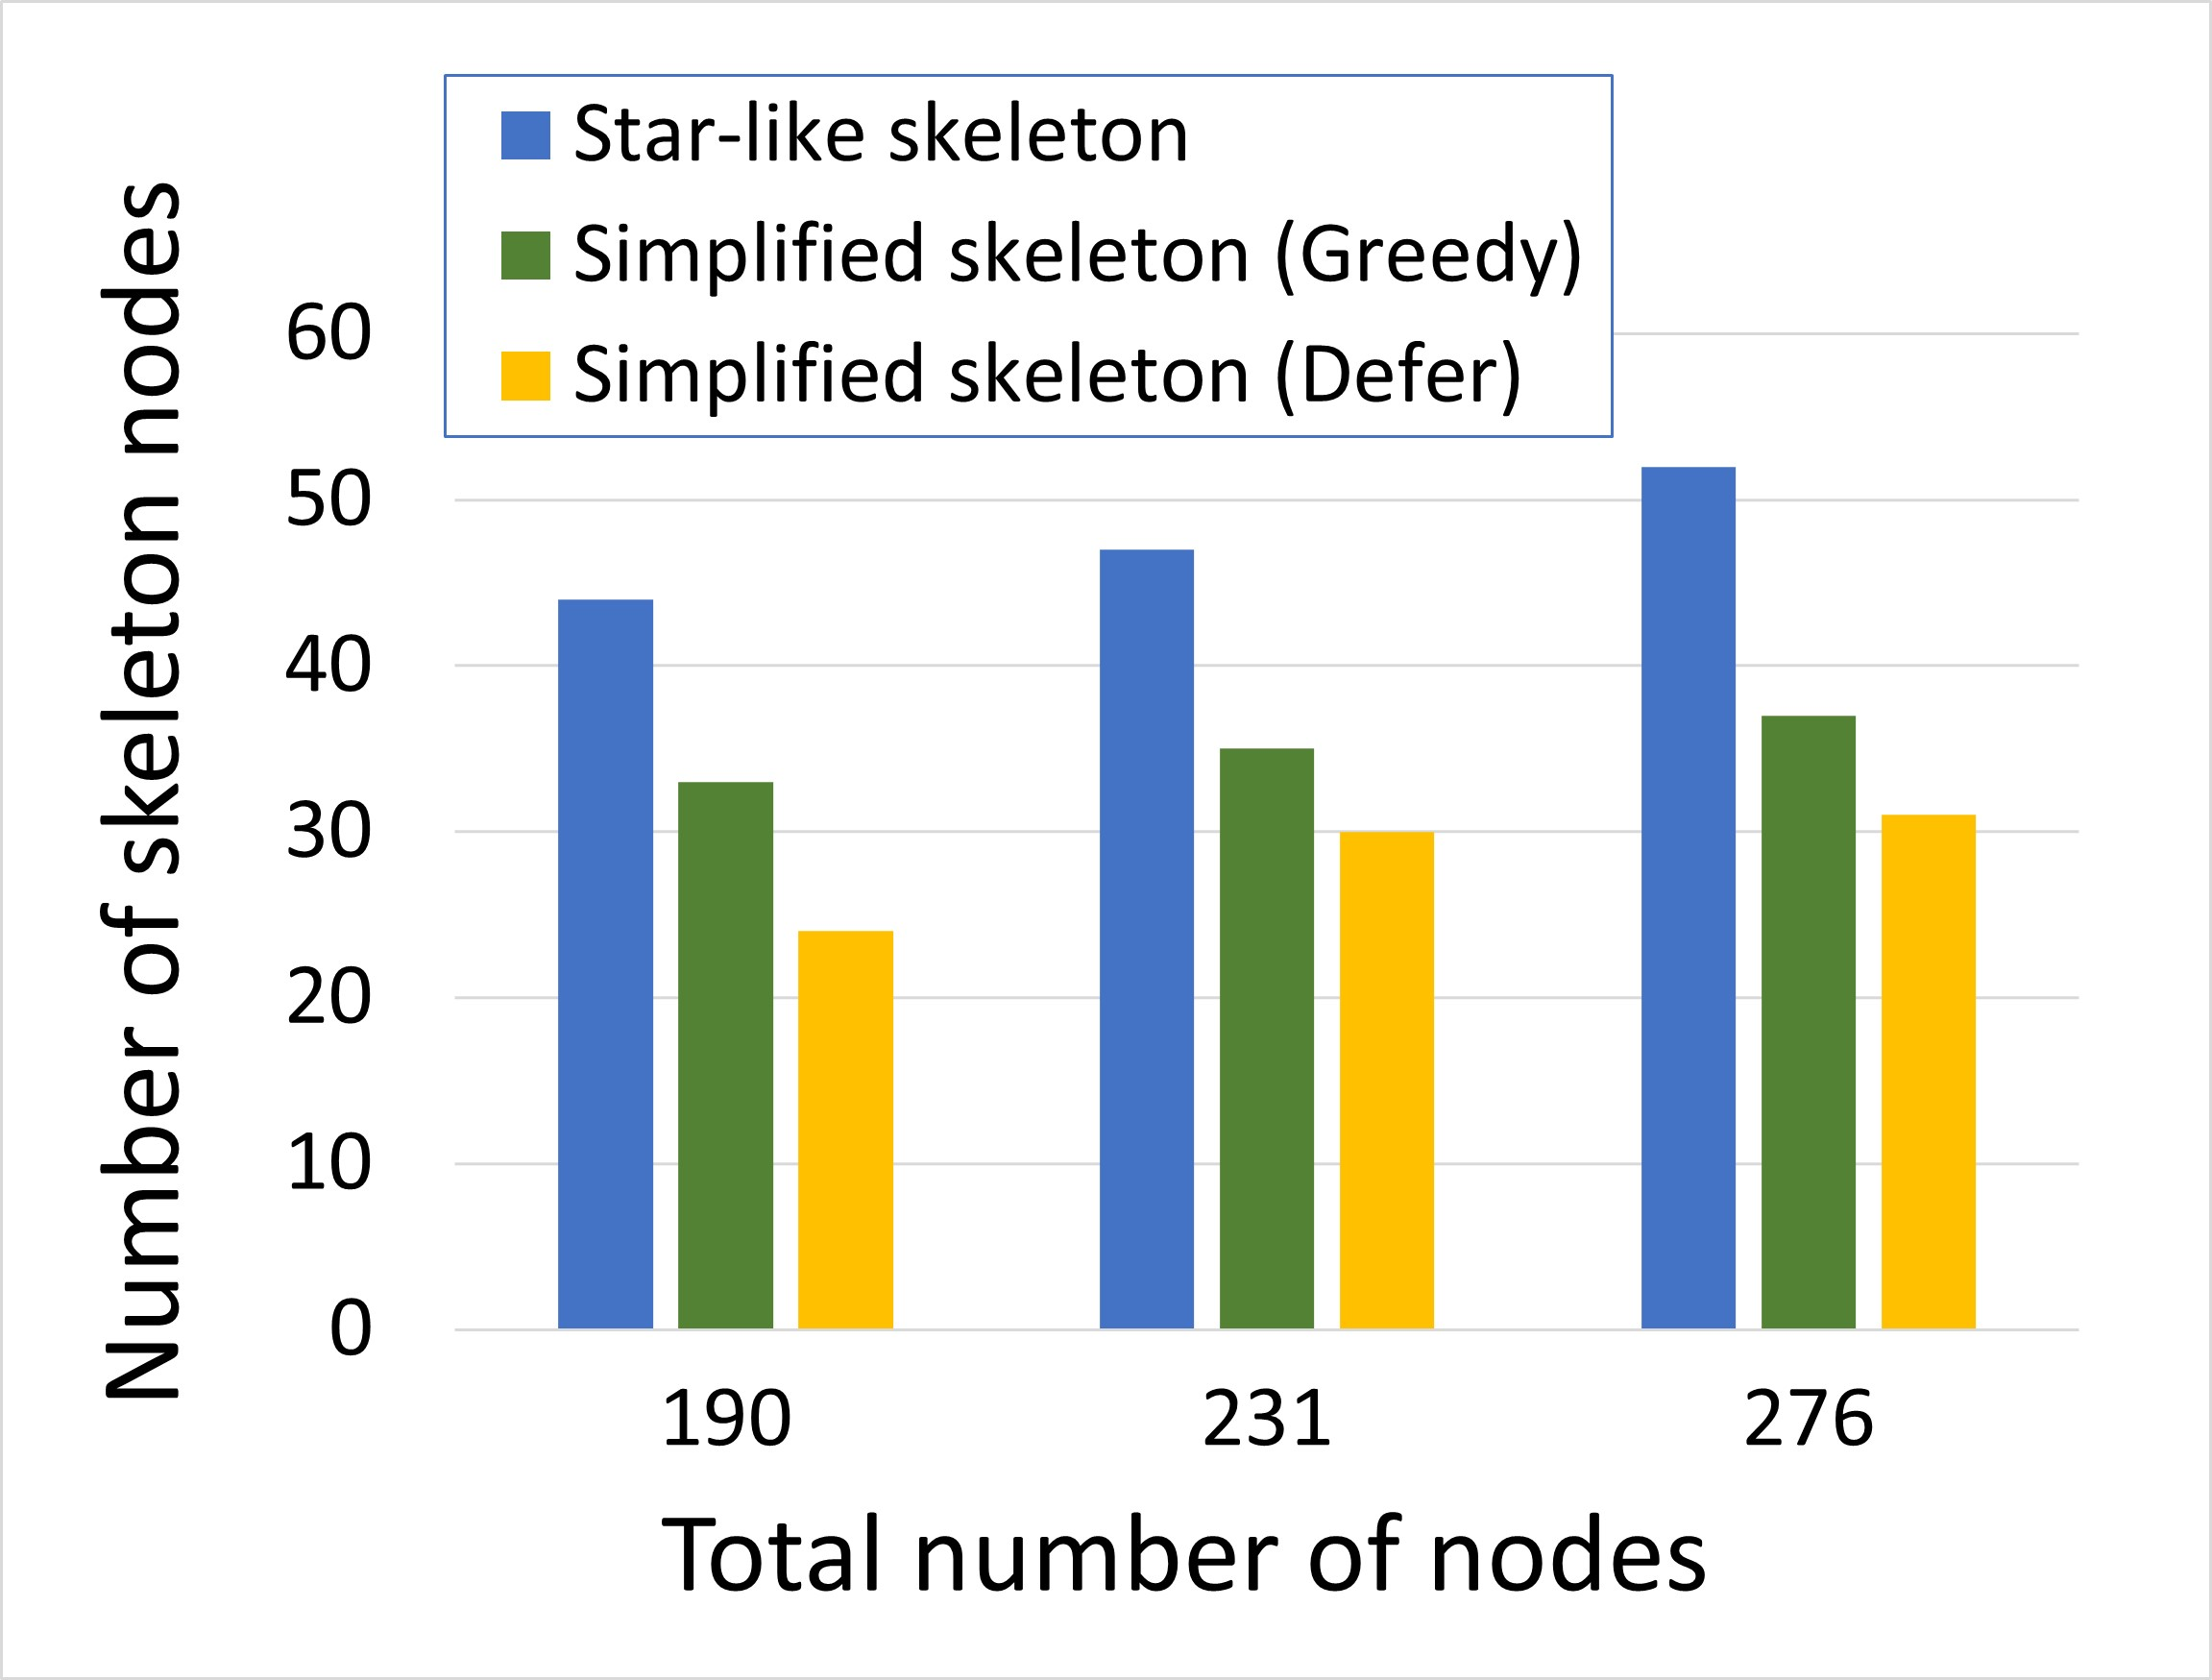
\includegraphics[width=0.8\textwidth]{images/results_skeleton_triagular.jpg}
        \caption{Triangular swarm formation}
    \end{subfigure}
\caption{Size of the skeletons}
\end{figure}
%=== figure === %

\subsection{Number of broadcast sources}

\paragraph{}
Figure 4.3(a) shows that, with the square swarm formation, Defer algorithm selects significantly less broadcast sources than Greedy with the star-like skeleton framework. Moreover, the simplified skeleton structure requires fewer broadcast sources than the star-like skeleton for both algorithms. On the other hand, as shown in Figure 4.3(b), different skeleton structures and algorithms do not have a noticeable effect on the number of broadcast sources required for the triangular swarm formation.

\paragraph{}
%=== figure === %
\begin{figure}[tbph]
    %\centering
    \begin{subfigure}{1\linewidth}
    \centering
        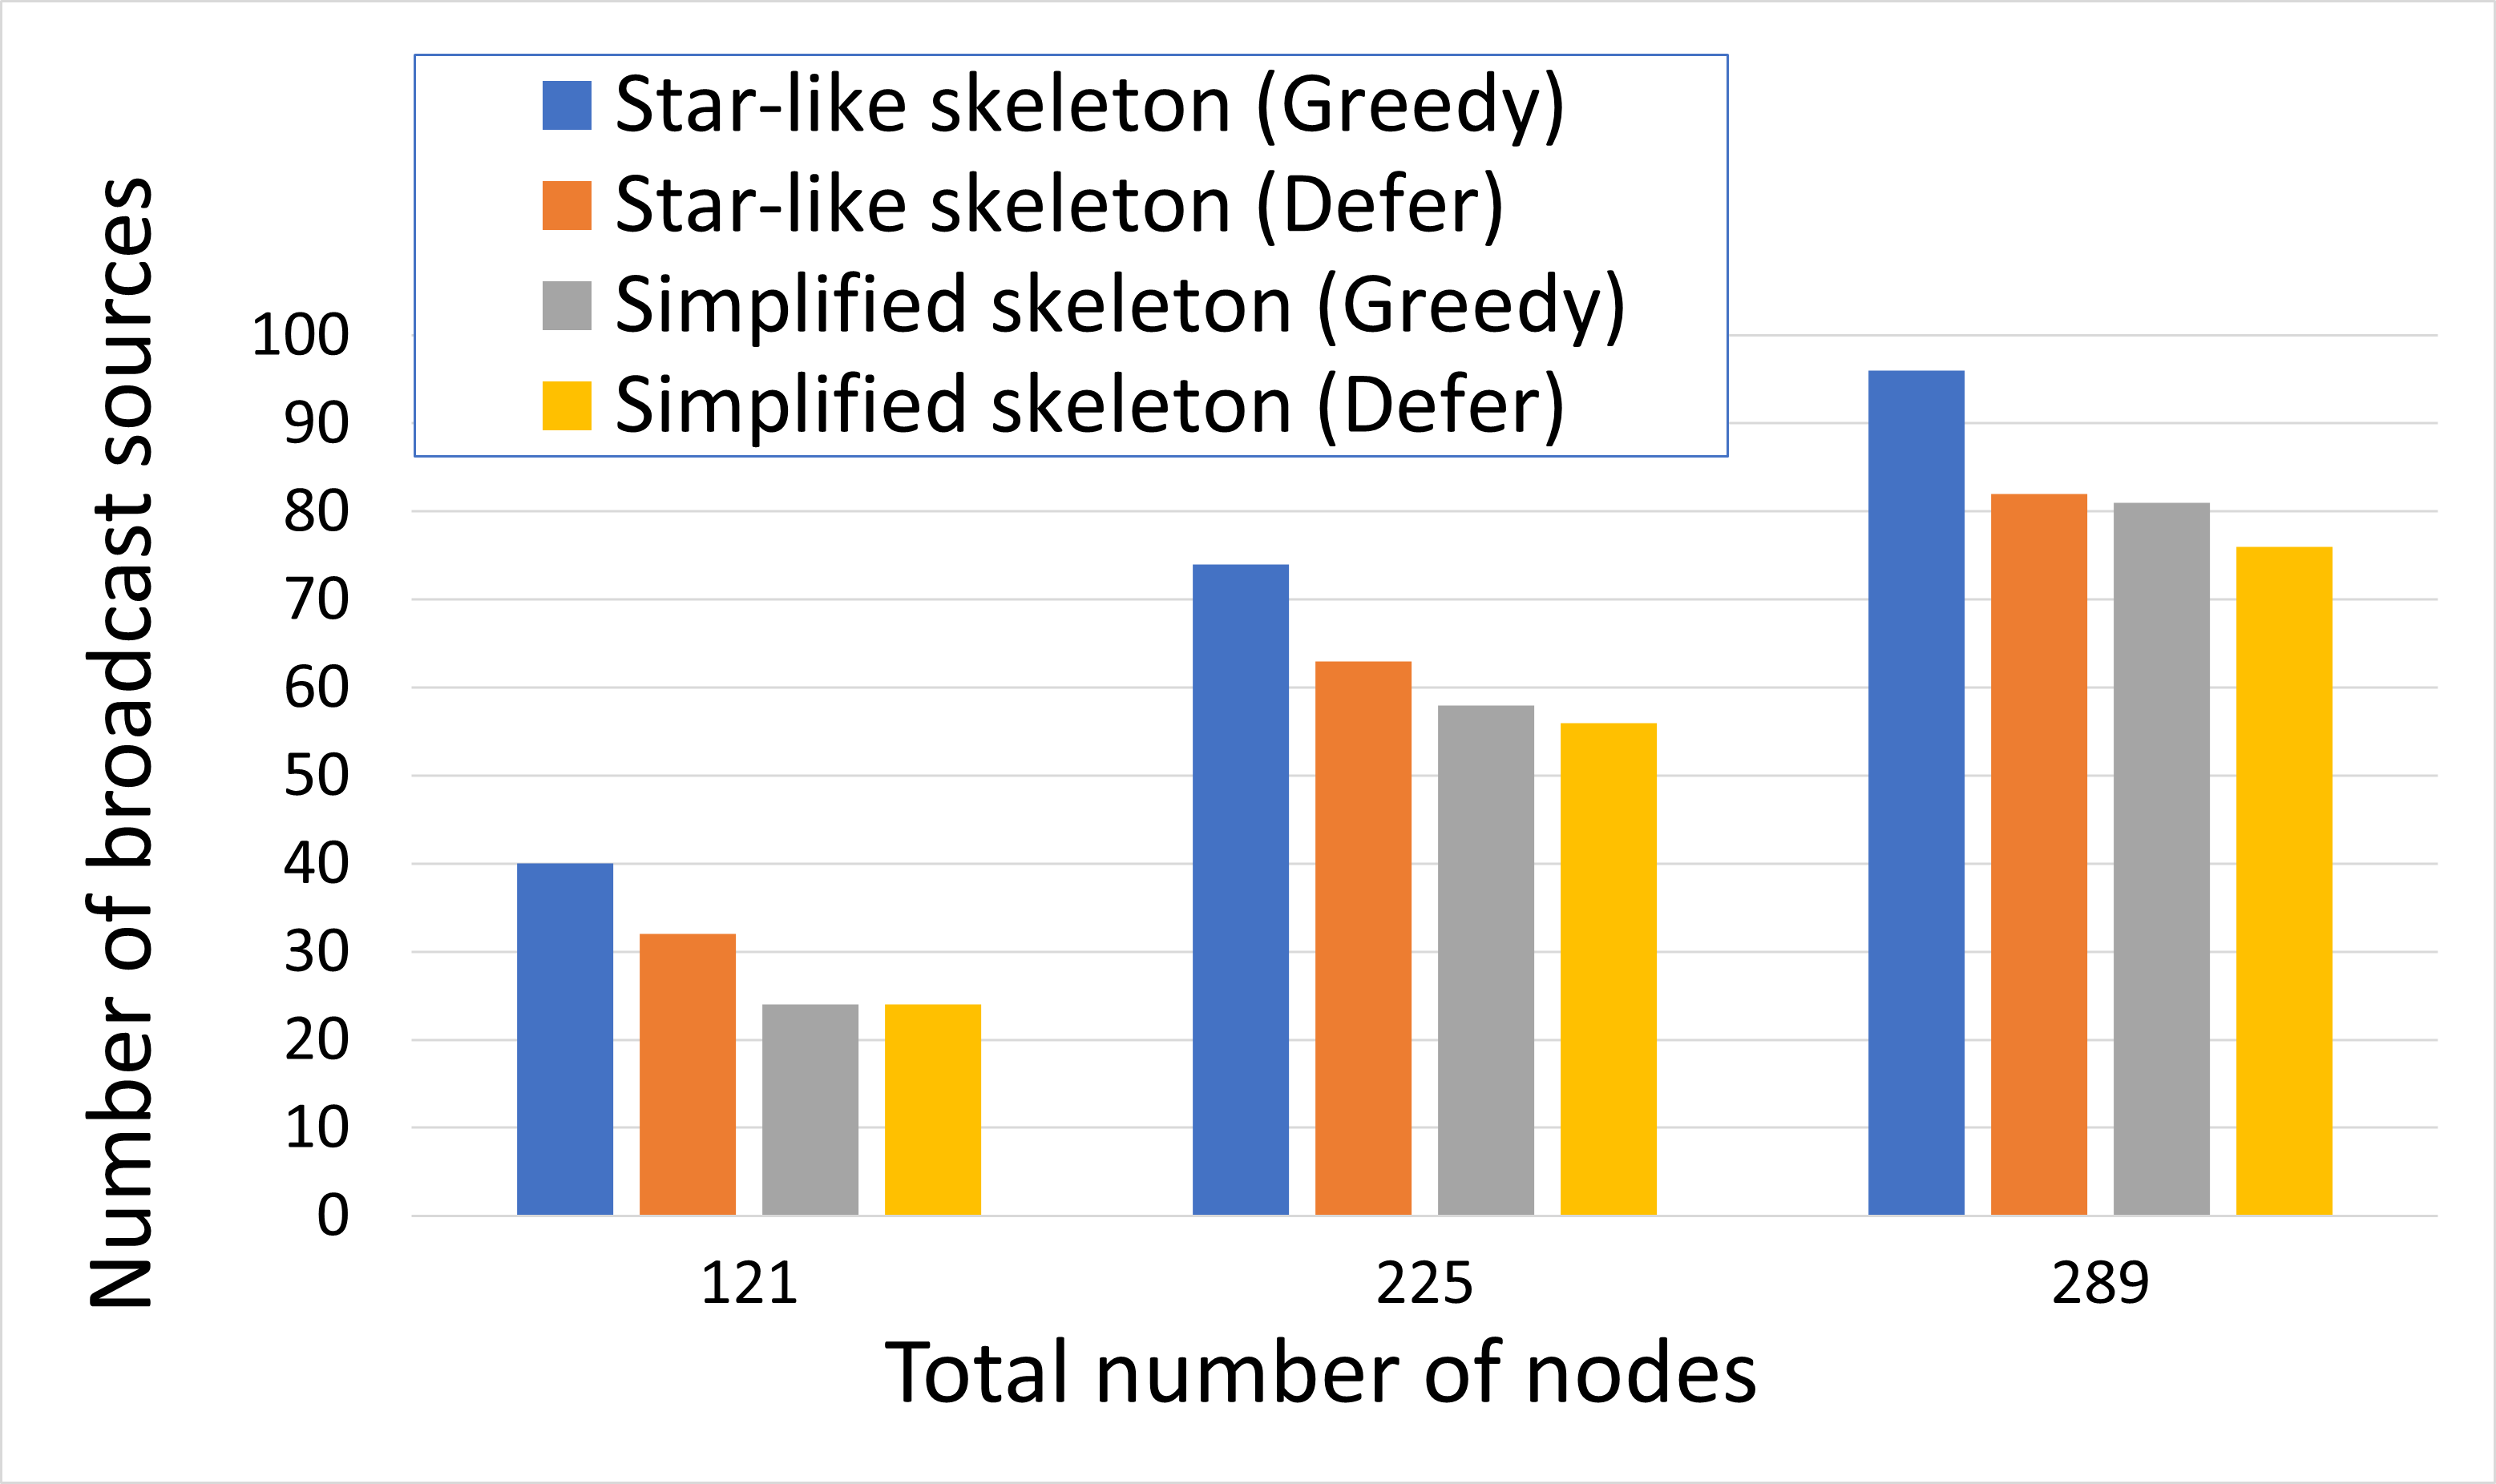
\includegraphics[width=0.8\textwidth]{images/results_broadcasts_square.png}
        \caption{Square swarm formation}
    \end{subfigure}
    
    \vspace{1cm}
    \begin{subfigure}{1\linewidth}
    \centering
        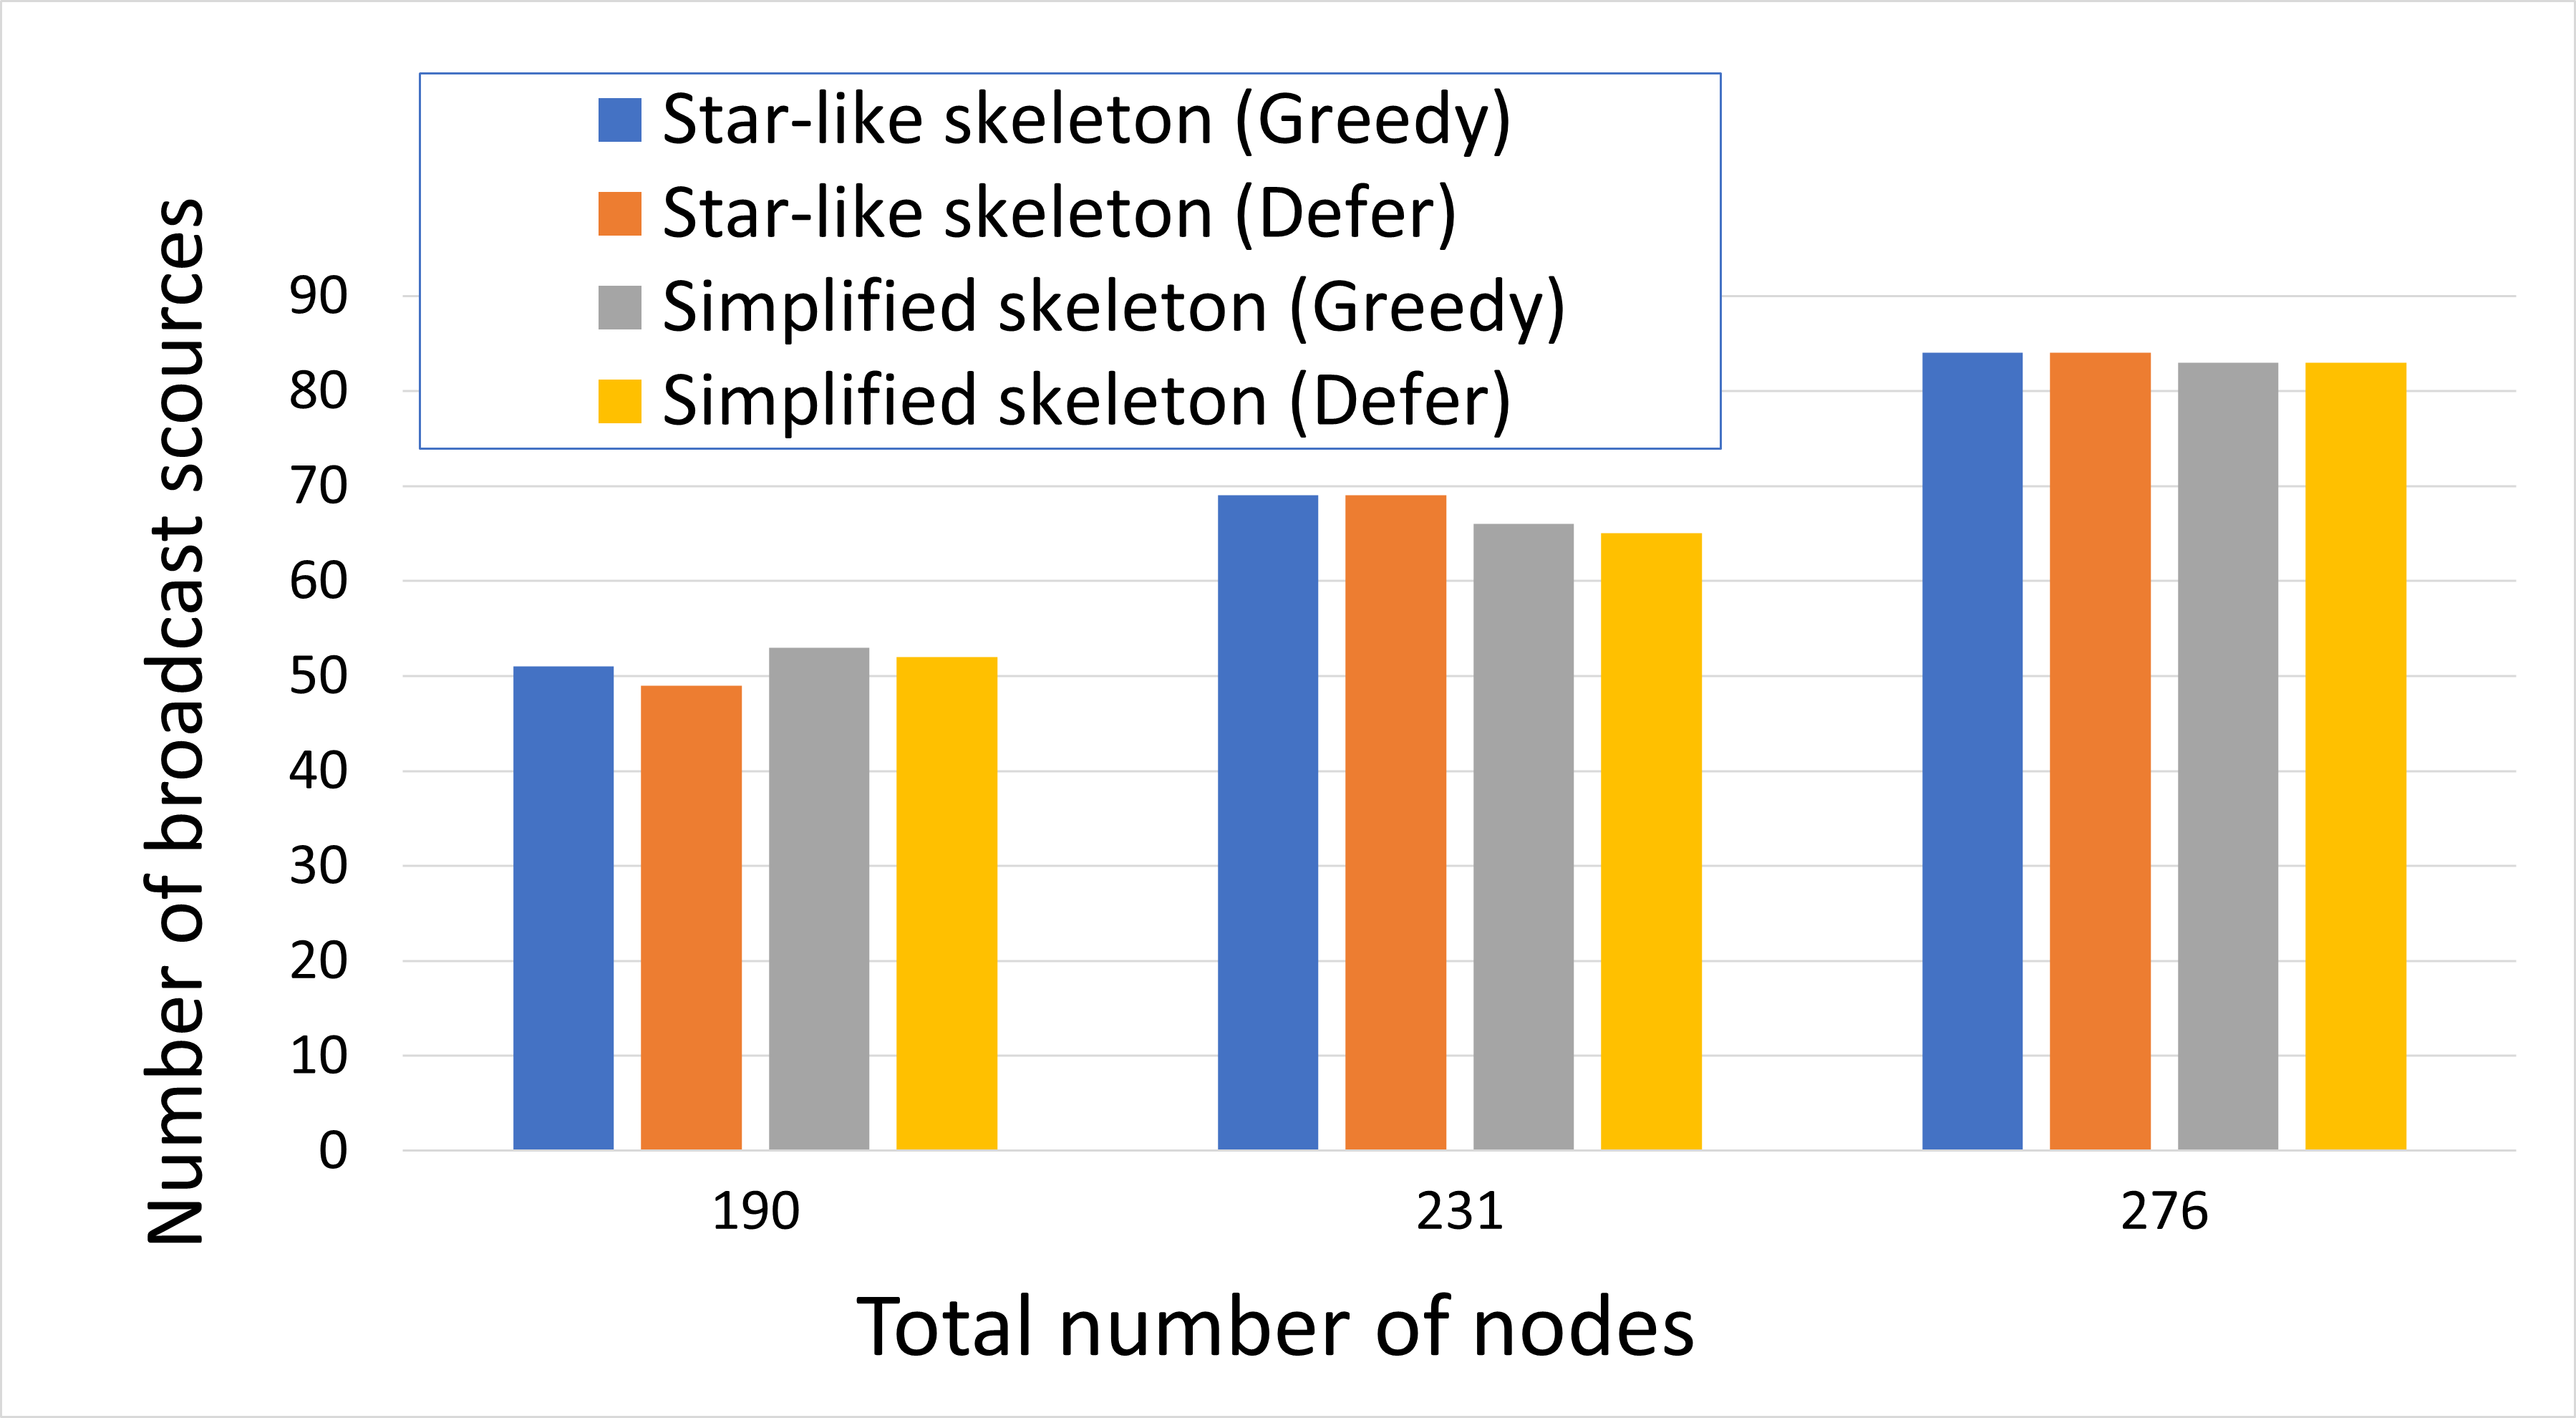
\includegraphics[width=0.8\textwidth]{images/results_broadcasts_triangular.png}
        \caption{Triangular swarm formation}
    \end{subfigure}
\caption{Number of broadcast sources}
\end{figure}
%=== figure === %

\subsection{Number of broadcast iterations}
\paragraph{}
The number of iterations represents the maximum number of hops required for the entire network to receive the message. Less hops means less hopes means lower end-to-end delay. Figure 4.4 shows our simplified skeletons effectively reduce the number of broadcast iterations required, especially for the square swarm formations. For the square swarm formations, simplifying the star-like skeleton using our adapted algorithm can save up to 60\% of the broadcast iterations required.


%=== figure === %
\begin{figure}[tbph]
    %\centering
    \begin{subfigure}{1\linewidth}
    \centering
        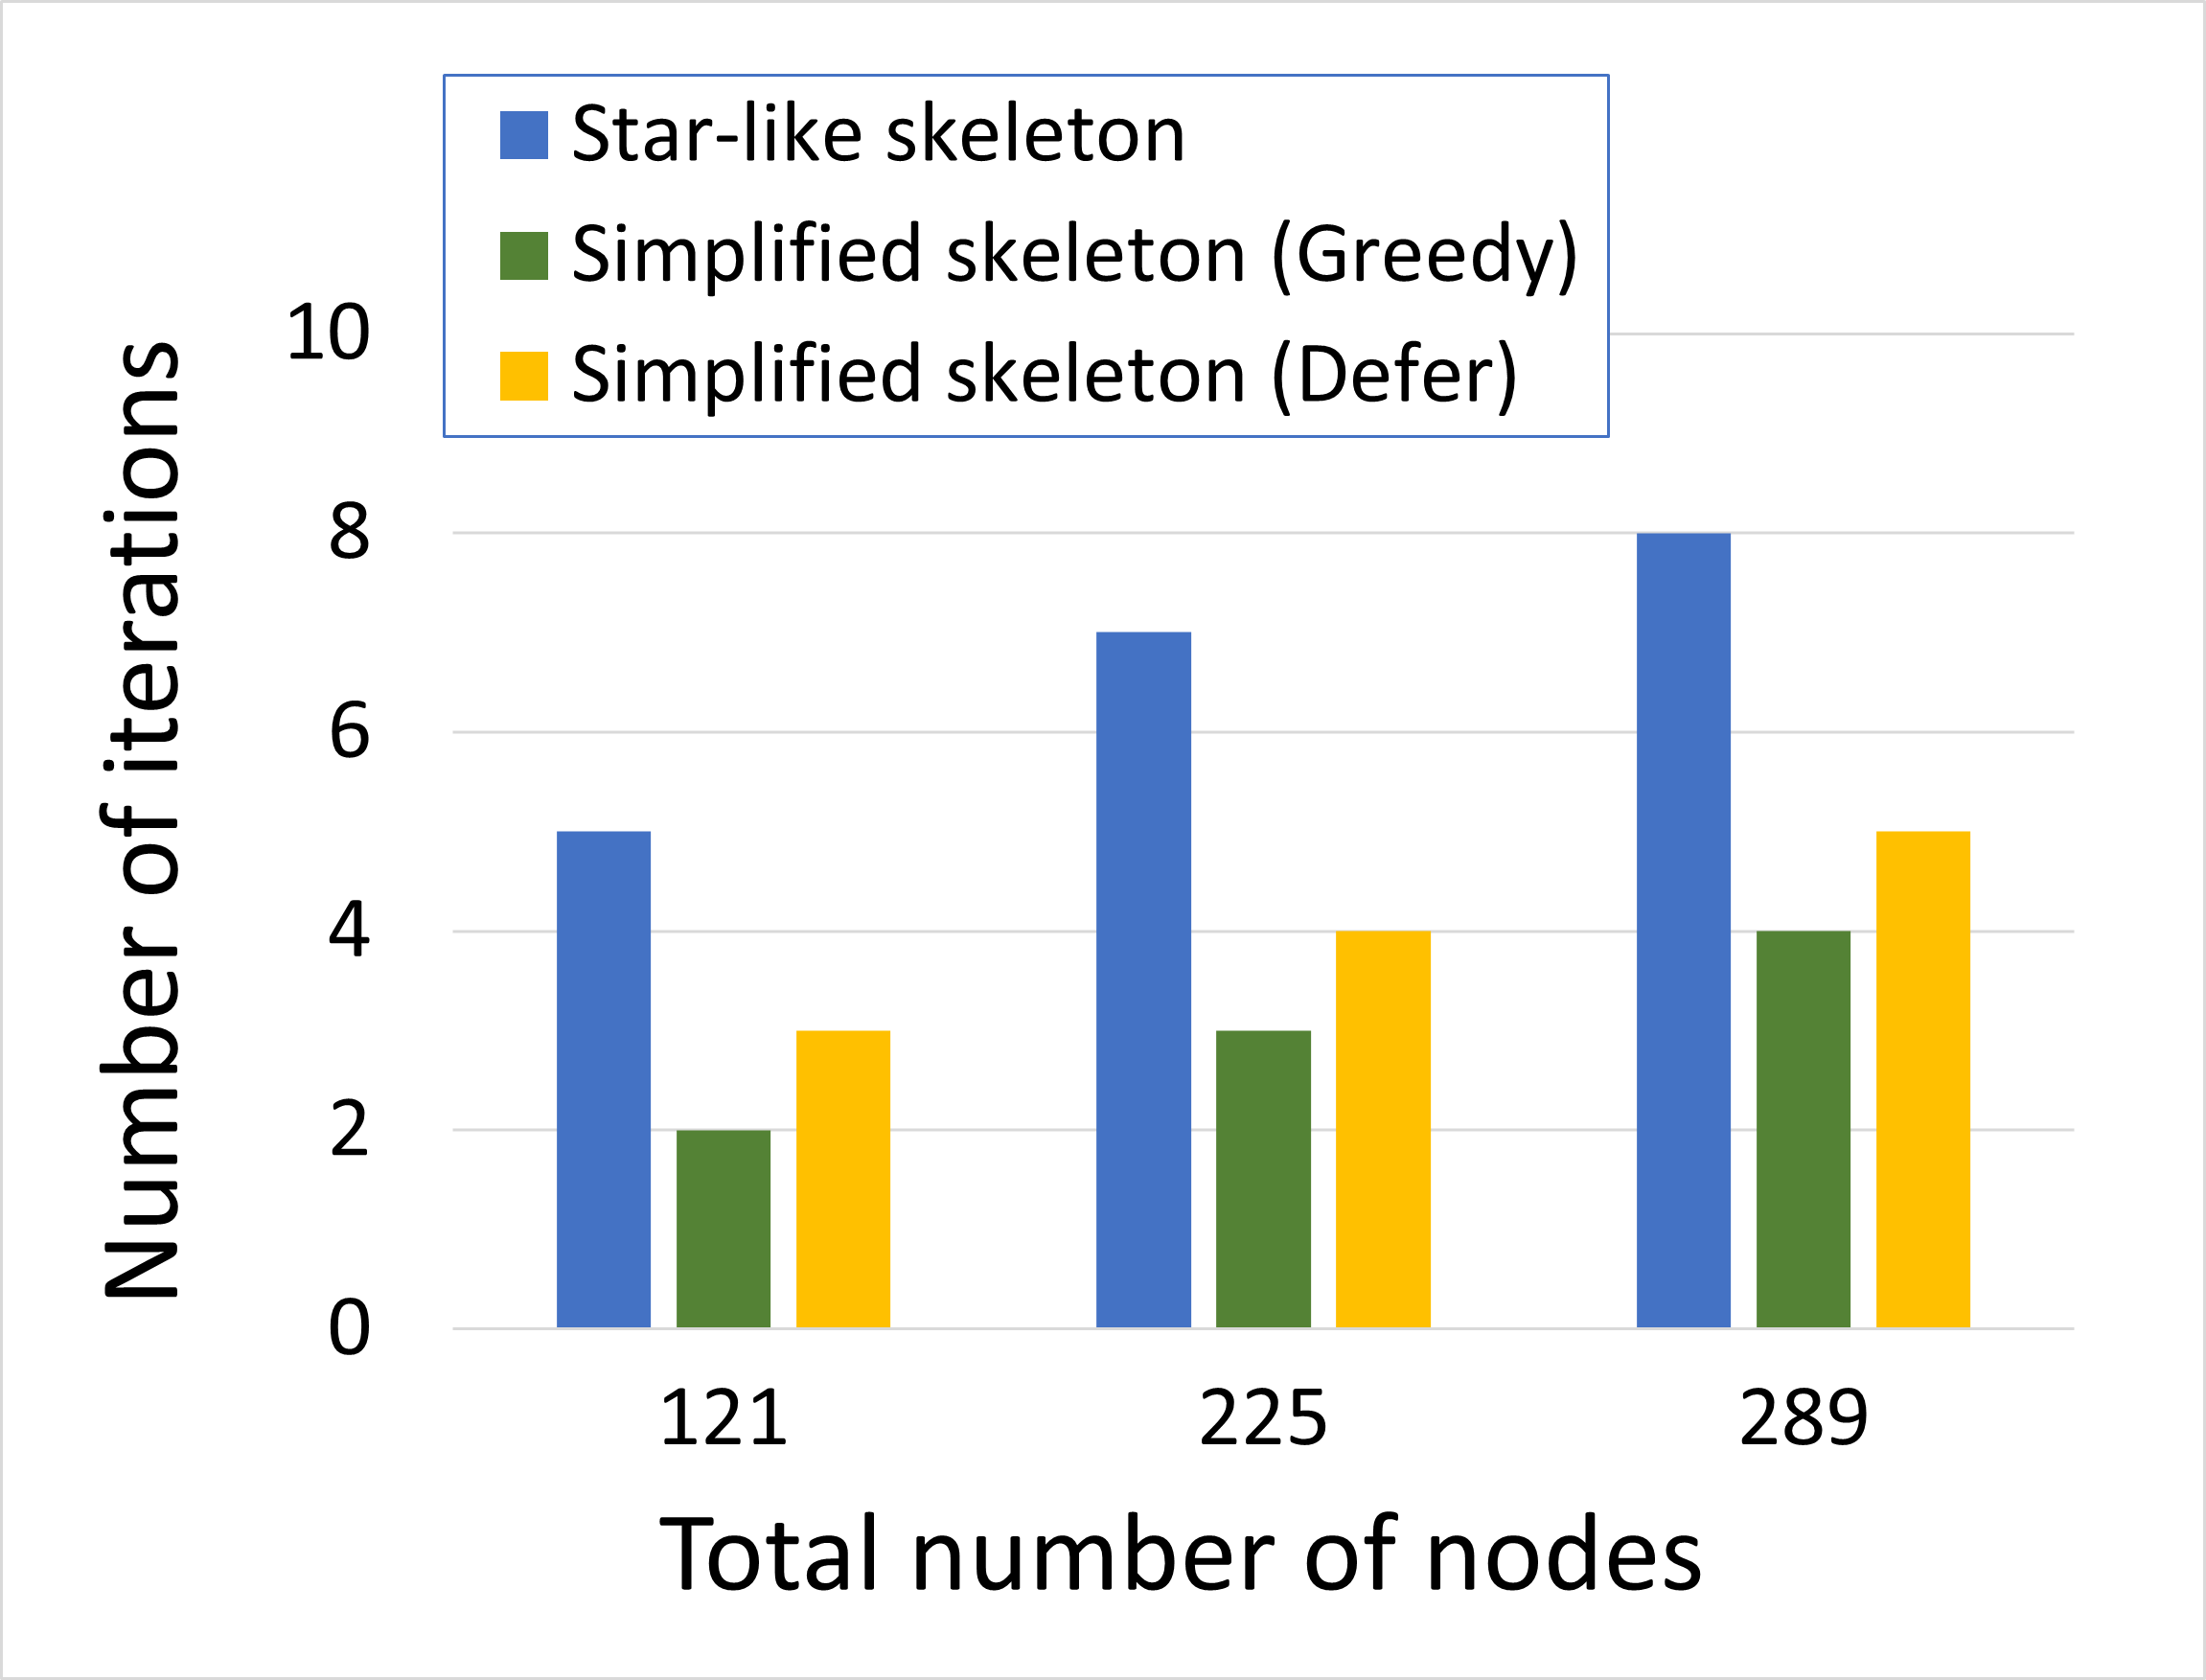
\includegraphics[width=0.8\textwidth]{images/results_iterations_square.png}
        \caption{Square swarm formation}
    \end{subfigure}
    
    \vspace{1cm}
    \begin{subfigure}{1\linewidth}
    \centering
        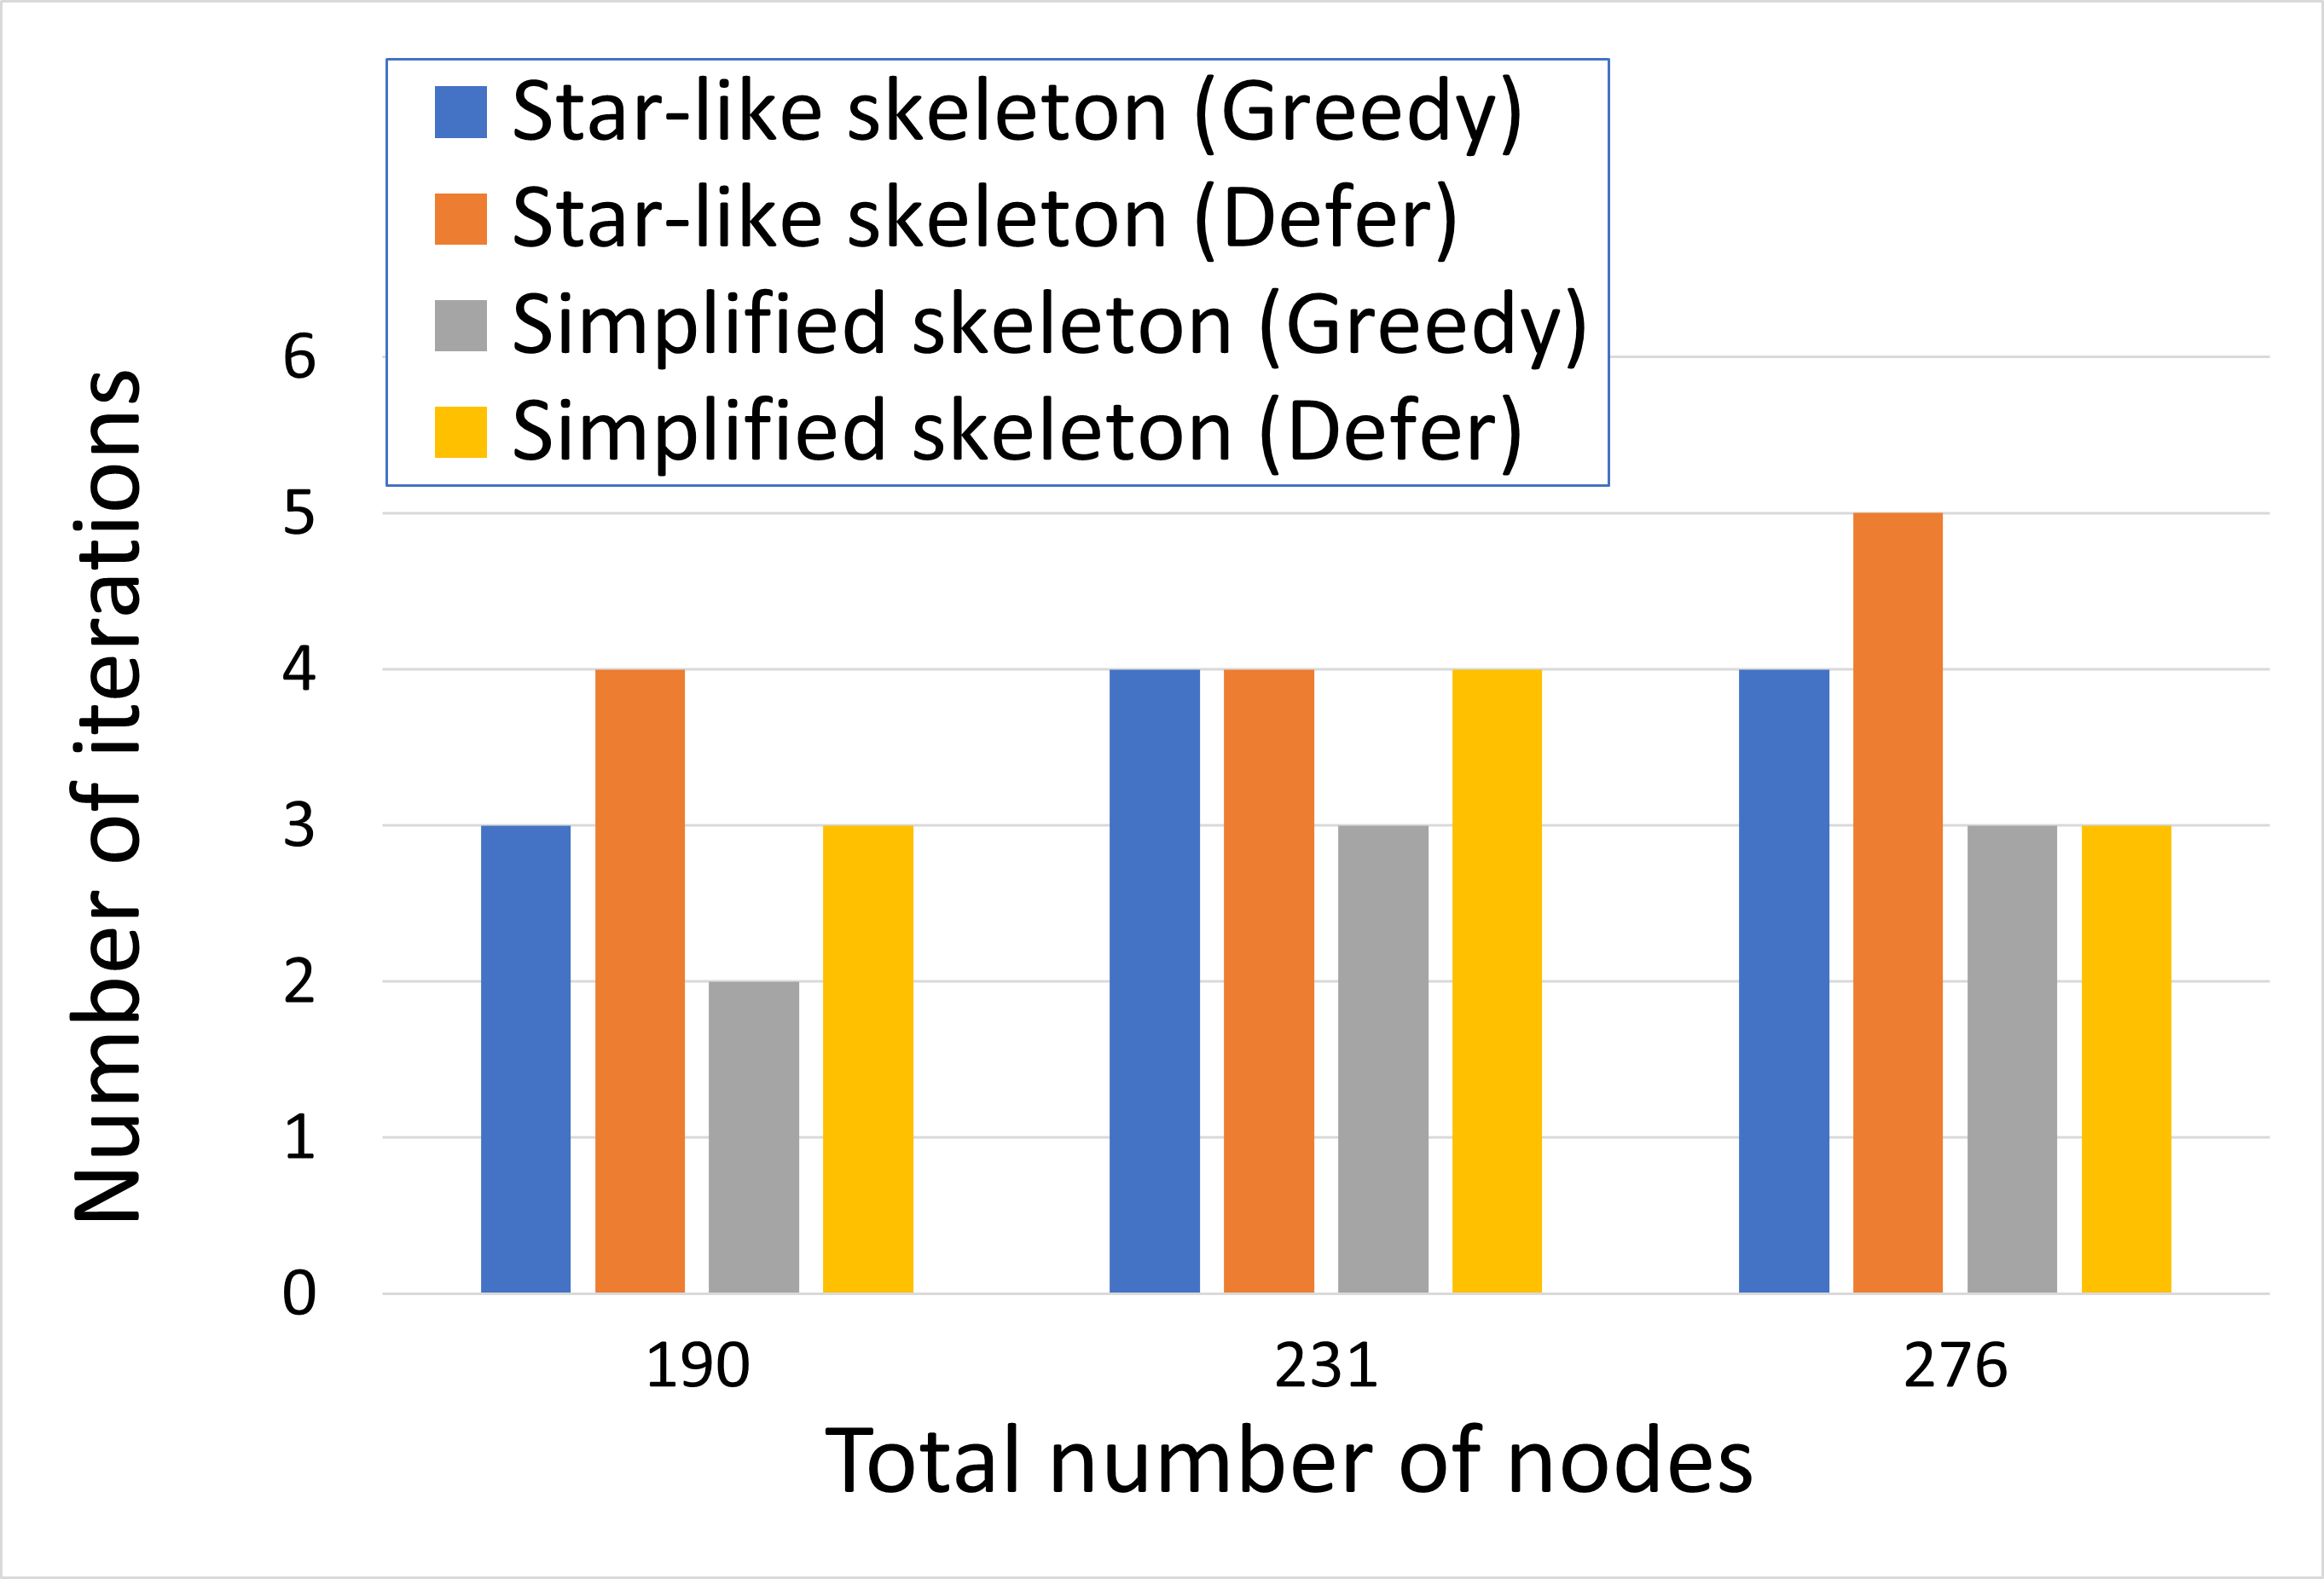
\includegraphics[width=0.8\textwidth]{images/results_iterations_triangular.png}
        \caption{Triangular swarm formation}
    \end{subfigure}
\caption{Number of broadcast iterations}
\end{figure}
%=== figure === %

%*------------------------------------------------------



%*------------------------------------------------------
\chapter{Conclusion}
\paragraph{}
In this thesis, we introduce the background and current state of small-size UAV swarm communicating. We also integrate the skeleton framework of \cite{ssr} into large-scale fixed-shape UAV swarm broadcast scenarios and apply two greedy-based source selection algorithms proposed by \cite{prose} onto the framework to investigate their performance. In addition, we adapt the algorithms to simplify the star-like framework making them more suitable for broadcast communications. The experimental results indicates that our method of simplifying the star-like skeleton can significantly lower the broadcasts costs by reducing skeleton nodes, the number of broadcasts, and the number broadcast iterations. The future research will investigate the application of the skeleton framework in a 3D dynamic UAV swarm network.

%*------------------------------------------------------


\addcontentsline{toc}{chapter}{Bibliography}
\bibliographystyle{IEEEtran}
\bibliography{references}

\end{document}

